\documentclass[12pt]{article}
\usepackage[utf8]{inputenc}
\usepackage[a4paper, margin=2cm]{geometry}
\usepackage{amsthm}
\usepackage{amsmath, amssymb}
\usepackage{circuitikz}
\usepackage{graphicx}
\usepackage{karnaugh-map}
\usepackage{newtxtext, newtxmath}
\usepackage{pgfplots}
\usepackage{tcolorbox}
\usepackage{tikz}
\usepackage{titlesec}
\usepackage{xcolor}
\usepackage{listings}
\usepackage{xeCJK}
\usetikzlibrary{patterns,arrows,decorations.pathmorphing}
\definecolor{lightblue}{RGB}{135, 206, 250}
\definecolor{commentgreen}{rgb}{0.25,0.5,0.35}
\definecolor{keywordblue}{rgb}{0.13,0.13,1}
\definecolor{stringmagenta}{rgb}{0.5,0,0.35}
\tcbuselibrary{skins,theorems}

\titleformat{\section}[block]{\Large\bfseries\centering}{}{0pt}{}
\titleformat{\subsection}[block]{\bfseries}{\thesubsection}{2pt}{}

\lstdefinestyle{verilogstyle}{
  language=Verilog,                % 设置语言
  backgroundcolor=\color{white},   % 背景色
  commentstyle=\color{commentgreen},% 注释样式
  keywordstyle=\color{keywordblue}, % 关键字样式
  numberstyle=\tiny\color{gray},    % 行号的样式
  stringstyle=\color{stringmagenta},% 字符串样式
  basicstyle=\ttfamily\small,      % 代码基本样式
  breakatwhitespace=false,         % 是否只在空白处换行
  breaklines=true,                 % 自动换行
  captionpos=b,                    % 标题位置（底部）
  keepspaces=true,                 % 保留空格
  numbers=left,                    % 行号的位置
  numbersep=5pt,                   % 行号与代码的距离
  showspaces=false,                % 是否显示空格
  showstringspaces=false,          % 字符串中的空格是否显示
  showtabs=false,                  % 是否显示制表符
  tabsize=2,                       % 制表符的宽度
  frame=single,                    % 边框样式
  rulecolor=\color{black}          % 边框颜色
}

% 创建一个新的listings环境
\lstnewenvironment{verilogcode}[1][]
{
  \lstset{style=verilogstyle, #1} % 使用Verilog样式，允许自定义设置
}{}

\newtcbtheorem[no counter]{proposition}{\large\hspace{-8pt}Proposition}{
  enhanced,
  colback=white,
  colframe=lightblue,
  left=12pt,
  right=12pt,
  top=24pt,
  bottom=24pt,
  fonttitle=\bfseries
}{prop}
\newtcbtheorem[]{question}{\large\hspace{-8pt}Question :}{
  enhanced,
  colback=white,
  colframe=black,
  left=12pt,
  right=12pt,
  top=24pt,
  bottom=24pt,
  fonttitle=\bfseries
}{qst}
\newenvironment{Answer}{
  \vspace{12pt}
  {\large\textbf{\textit{\hspace{-12pt}Answer:}}}\par
  \vspace{8pt}
} {\vspace{24pt}}
\newenvironment{Proof}{
  \vspace{12pt}
  {\large\textbf{\textit{\hspace{-12pt}Proof:}}}\par
  \vspace{8pt}
} {\vspace{24pt}}

\title{DCHw1}
\author{Miki-Riako }
\date{\today}
\begin{document}

\begin{question}{}{}
  6-3 Analyze and write the functions and the equation.
\end{question}
\begin{Answer}
易得功能是二位加法。

由于D触发器的特征方程，
得到驱动方程：
$$D_0=\overline {Q^n_0}$$
$$D_1=Q^n_1\oplus Q^n_0$$

代入得到状态方程：

$$Q^{n+1}_0=\overline {Q^n_0}$$
$$Q^{n+1}_1=Q^n_1\oplus Q^n_0$$

输出方程即为：

$$F=Q^n_0Q^n_1$$

状态转化图为：

\begin{center}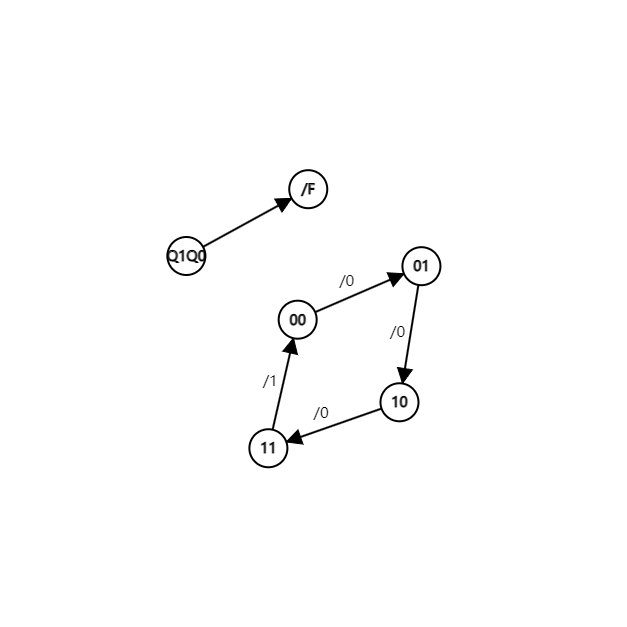
\includegraphics[width=0.4\textwidth]{image/graph_1.png}\end{center}
\end{Answer}

\begin{question}{}{}
  6-4 Analyze and write the functions and the equation.
\end{question}
\begin{Answer}
易得功能是7进制计数器。

由于JK触发器的特征方程，
得到驱动方程：
$$J_0=\overline {Q^n_2Q^n_1},\;\;K_0=1$$
$$J_1=Q^n_0,\;\;K_1=\overline {\overline {Q^n_0}\;\overline {Q^n_2}}$$
$$J_2=1,\;\;K_2=1$$

代入得到状态方程：

$$Q^{n+1}_0=\overline {Q^n_2Q^n_1}\;\overline {Q^n_0}$$
$$Q^{n+1}_1=Q^n_0\;\overline {Q^n_1}+\overline {Q^n_0}\;\overline {Q^n_2}\;Q^n_1$$
$$Q^{n+1}_2=\overline {Q^n_2},\;\;Q_1\downarrow $$

时钟方程为：

$$CLK_0=CP$$
$$CLK_1=CP$$
$$CLK_2=Q^n_1$$

状态转化图为：

\begin{center}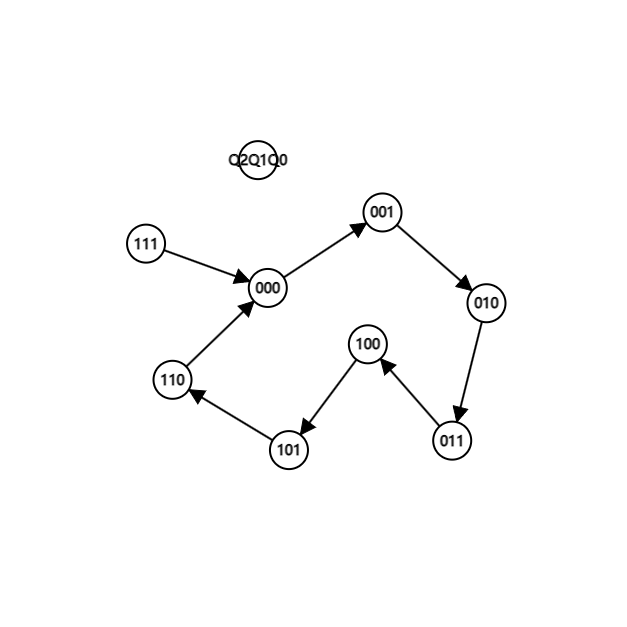
\includegraphics[width=0.4\textwidth]{image/graph_2.png}\end{center}
\end{Answer}

\begin{question}{}{}
  6-7 Design a 6-bit adder using JK.
\end{question}
\begin{Answer}
可知状态转化图为：

\begin{center}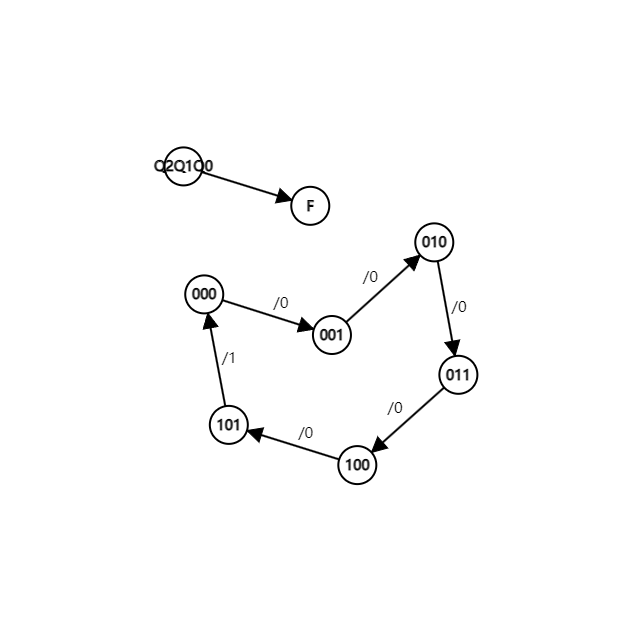
\includegraphics[width=0.4\textwidth]{image/graph_3.png}\end{center}

绘制卡诺图，得到：

\noindent\begin{minipage}[t]{0.5\textwidth}
\begin{center}\begin{karnaugh-map}[4][2][1][$Q^n_1Q^n_0$][$Q^n_2$]
  \manualterms{001, 010, 011, 100, 101, 000, -, -}
\end{karnaugh-map}\end{center}
\end{minipage}\begin{minipage}[t]{0.5\textwidth}
\begin{center}\begin{karnaugh-map}[4][2][1][$Q^n_1Q^n_0$][$Q^n_2$]
  \minterms{5}
  \maxterms{0,1,2,3,4}
  \indeterminants{6,7}
  \implicant{5}{7}
\end{karnaugh-map}\end{center}
\end{minipage}

由卡诺图得到状态方程与输出方程：

$$Q^{n+1}_0=\overline {Q^n_0}$$
$$Q^{n+1}_1=\overline {Q^n_2}\;\overline {Q^n_1}\;Q^n_0+Q^n_1\overline {Q^n_0}$$
$$Q^{n+1}_2=Q^n_2\overline {Q^n_0}+\overline {Q^n_2}Q^n_1Q^n_0$$
$$F=Q^n_2Q^n_0$$

由于JK触发器的特征方程，
得到驱动方程：
$$J_0=1,\;\;K_0=1$$
$$J_1=\overline {Q^n_2}Q^n_0,\;\;K_1=Q^n_0$$
$$J_2=Q^n_1Q^n_0,\;\;K_2=Q^n_0$$

得到逻辑图如图所示：
\begin{center}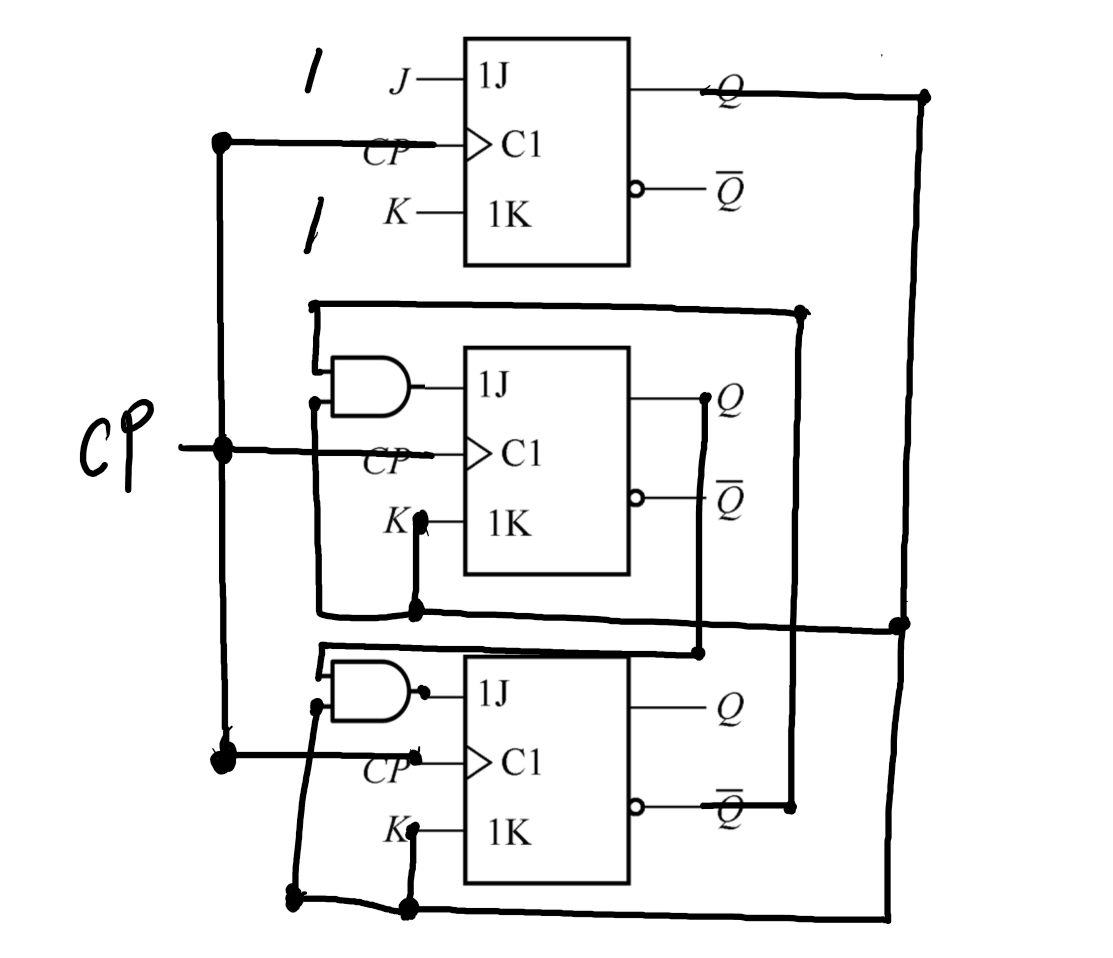
\includegraphics[width=0.4\textwidth]{image/electrical_14.png}\end{center}
\end{Answer}

\begin{question}{}{}
  6-8 Design a 12-bit adder using D.
\end{question}
\begin{Answer}
可知状态转化图为：

\begin{center}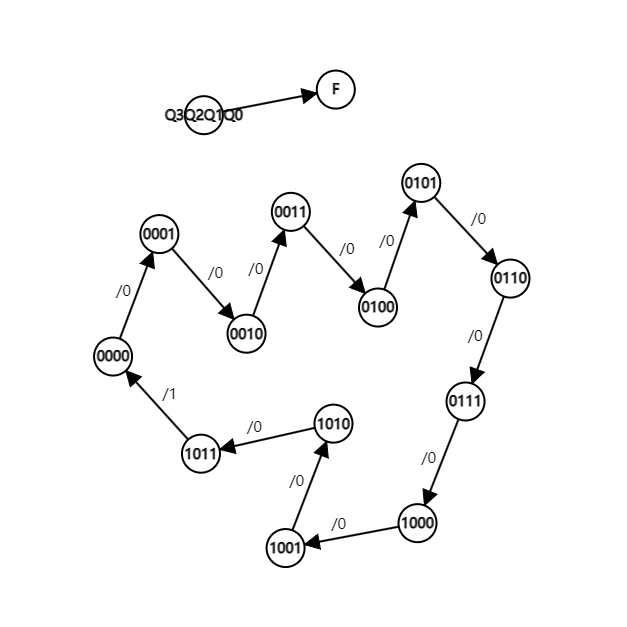
\includegraphics[width=0.4\textwidth]{image/graph_4.png}\end{center}

绘制卡诺图，得到：

\noindent\begin{minipage}[t]{0.5\textwidth}
\begin{center}\begin{karnaugh-map}[4][4][1][$Q^n_1Q^n_0$][$Q^n_3Q^n_2$]
  \manualterms{0001, 0010, 0011, 0100, 0101, 0110, 0111, 1000, 1001, 1010, 1011, 0000, -, -, -, -}
\end{karnaugh-map}\end{center}
\end{minipage}\begin{minipage}[t]{0.5\textwidth}
\begin{center}\begin{karnaugh-map}[4][4][1][$Q^n_1Q^n_0$][$Q^n_3Q^n_2$]
  \minterms{11}
  \maxterms{0,1,2,3,4,5,6,7,8,9,10}
  \indeterminants{12,13,14,15}
  \implicant{15}{11}
\end{karnaugh-map}\end{center}
\end{minipage}

由卡诺图得到状态方程与输出方程：

$$Q^{n+1}_0=\overline {Q^n_0}$$
$$Q^{n+1}_1=\overline {Q^n_1}\;Q^n_0+Q^n_1\overline {Q^n_0}$$
$$Q^{n+1}_2=Q^n_2\overline {Q^n_0}+Q^n_2\overline {Q^n_1}+\overline {Q^n_3}\;\overline {Q^n_2}Q^n_1Q^n_0$$
$$Q^{n+1}_3=Q^n_3\overline {Q^n_0}+Q^n_3\overline {Q^n_1}+Q^n_2Q^n_1Q^n_0$$
$$F=Q^n_3Q^n_1Q^n_0$$

由于D触发器的特征方程，
得到驱动方程：

$$D^{n+1}_0=\overline {Q^n_0}$$
$$D^{n+1}_1=\overline {Q^n_1}\;Q^n_0+Q^n_1\overline {Q^n_0}$$
$$D^{n+1}_2=Q^n_2\overline {Q^n_0}+Q^n_2\overline {Q^n_1}+\overline {Q^n_3}\;\overline {Q^n_2}Q^n_1Q^n_0$$
$$D^{n+1}_3=Q^n_3\overline {Q^n_0}+Q^n_3\overline {Q^n_1}+Q^n_2Q^n_1Q^n_0$$

得到逻辑图如图所示：
\begin{center}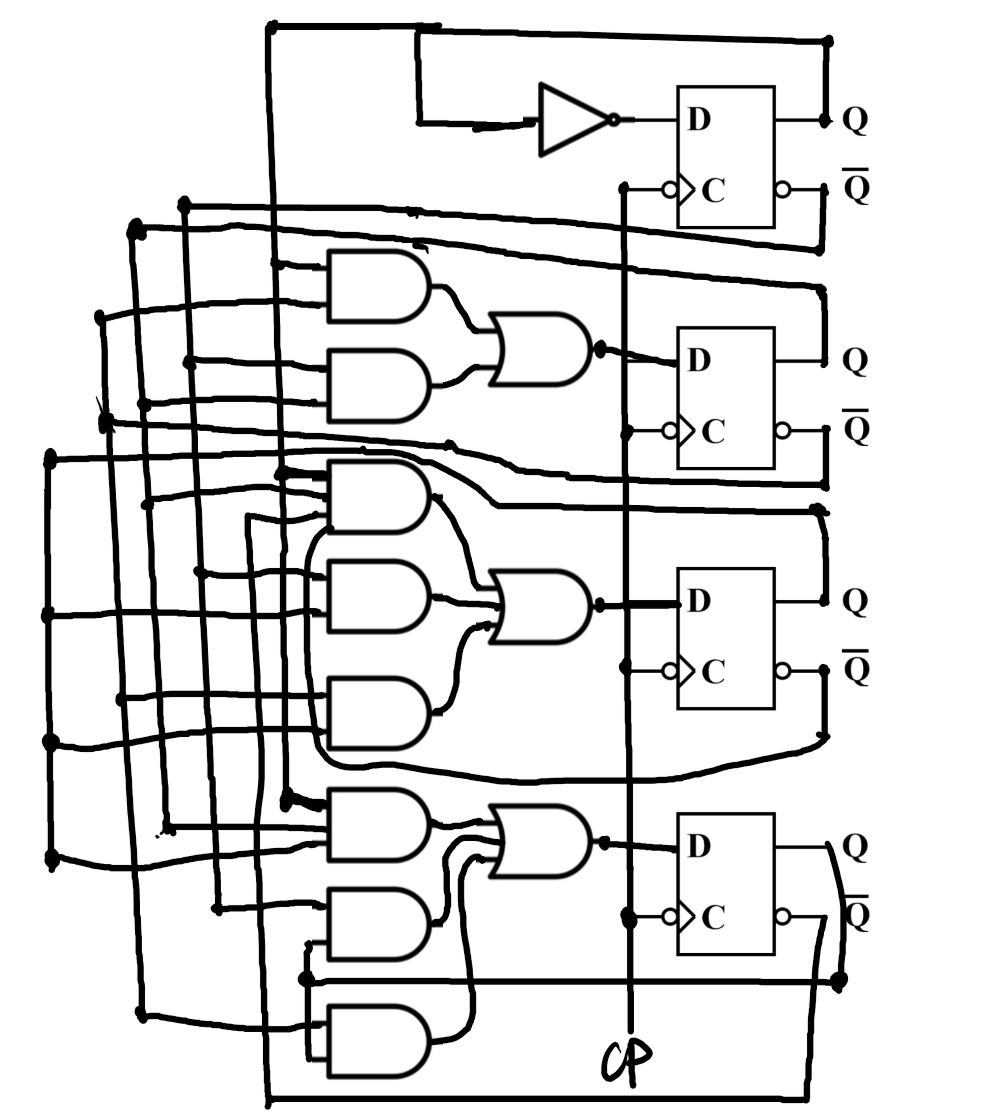
\includegraphics[width=0.4\textwidth]{image/electrical_15.png}\end{center}
\end{Answer}

\begin{question}{}{}
  6-11 Analyze the functions.
\end{question}
\begin{Answer}
C=1为2进制，C=0为4进制：

C=1:

载入0100，计数得到0101此时由于Load载入，回到载入0100，以此往复。
此时两个状态为二进制。

C=0：

载入0010，计数得到0011，计数得到0100，计数得到0101此时由于Load载入，回到载入0100，以此往复。
此时四个状态为四进制。
\end{Answer}

\begin{question}{}{}
  6-12 Analyze the functions.
\end{question}
\begin{Answer}
137进制计数器：

由于Q3连接了下一器件的CP，所以只有在Q3下降沿时下一器件计数。
第一器件是16进制计数器，只有在1111计数增一时得到0000才使得下一位计数增一。
最后，两个器件的Q3都为1时输出复位，即10001000时复位。
故器件是137进制计数器。
\end{Answer}

\begin{question}{}{}
  6-14 Analyze the functions.
\end{question}
\begin{Answer}
52进制计数器：

器件一将从1100计数到1111后，向下一器件发送一个计数信号增一。
之后器件一将从0000计数到1111后，才会向下一器件发送一个计数信号增一。
器件二从0011计数到1111后进位输出初始化两器件。
故进制为4+16*11=180，180进制计数器。
\end{Answer}

\begin{question}{}{}
  6-15 Build 11-bit adder.
\end{question}
\begin{Answer}
\begin{center}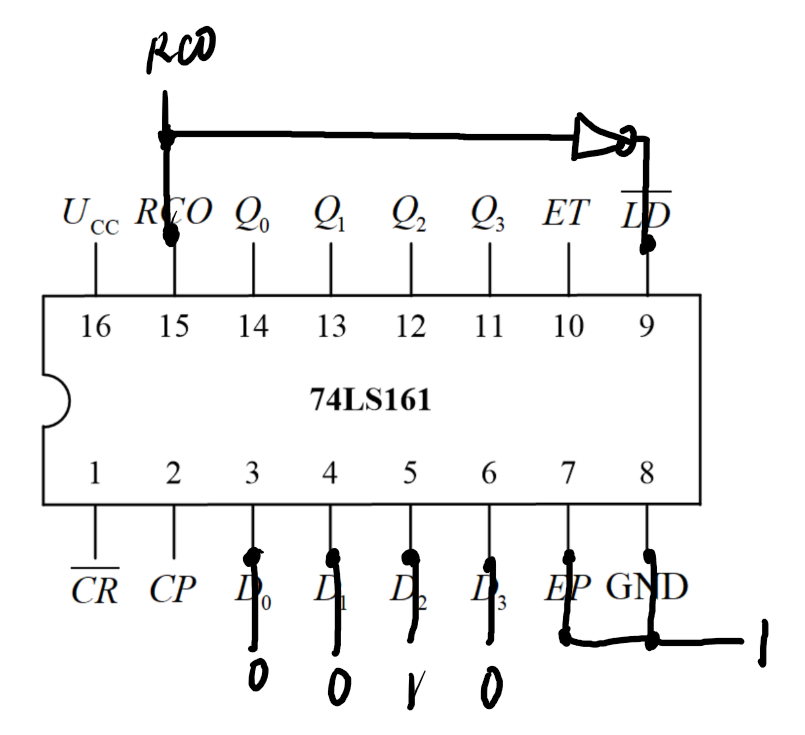
\includegraphics[width=0.4\textwidth]{image/electrical_16.png}\end{center}
\end{Answer}

\begin{question}{}{}
  6-18 Design 365-bit adder.
\end{question}
\begin{center}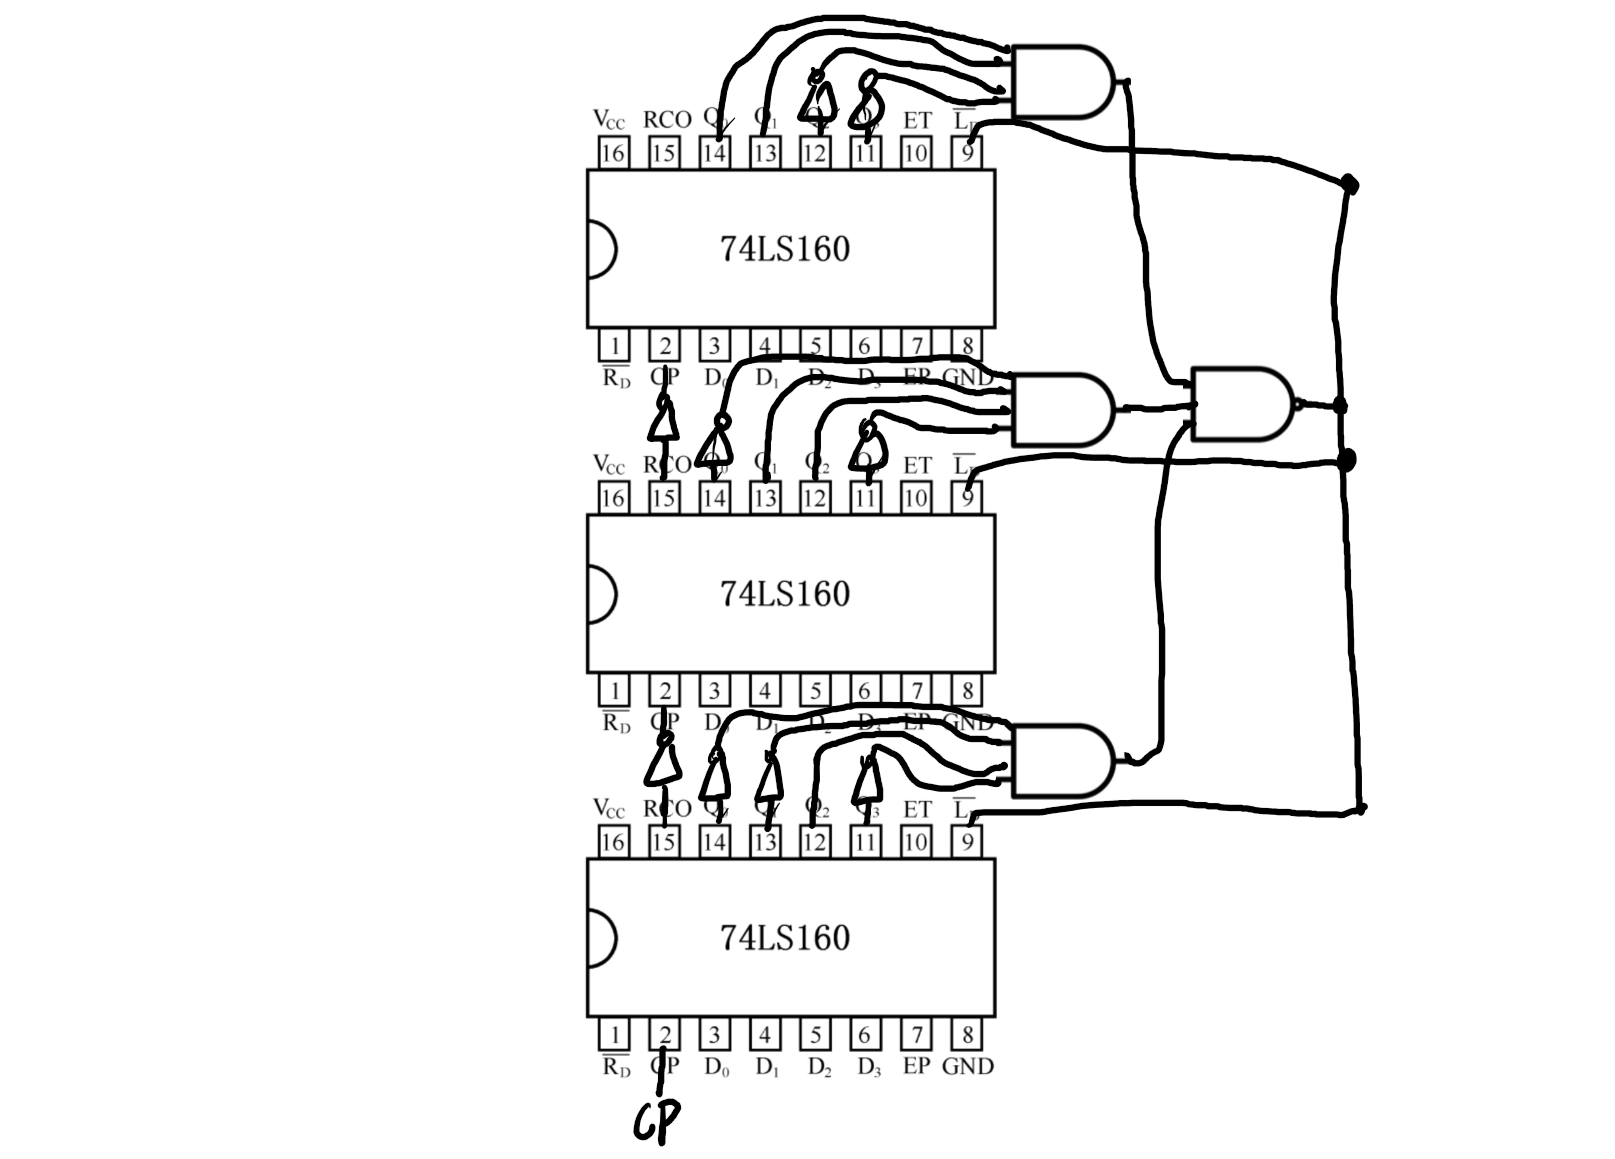
\includegraphics[width=0.4\textwidth]{image/electrical_17.png}\end{center}
\begin{Answer}

\end{Answer}

\begin{question}{}{}
  6-20 Design sequence generator.
\end{question}
\begin{Answer}
可知状态转化图为：

\begin{center}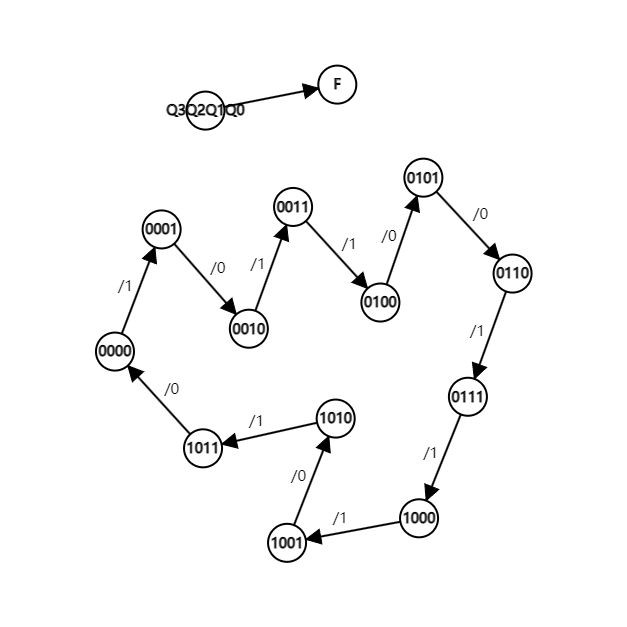
\includegraphics[width=0.4\textwidth]{image/graph_5.png}\end{center}

绘制卡诺图，得到：

\noindent\begin{minipage}[t]{0.5\textwidth}
\begin{center}\begin{karnaugh-map}[4][4][1][$Q^n_1Q^n_0$][$Q^n_3Q^n_2$]
  \manualterms{0001, 0010, 0011, 0100, 0101, 0110, 0111, 1000, 1001, 1010, 1011, 0000, -, -, -, -}
\end{karnaugh-map}\end{center}
\end{minipage}\begin{minipage}[t]{0.5\textwidth}
\begin{center}\begin{karnaugh-map}[4][4][1][$Q^n_1Q^n_0$][$Q^n_3Q^n_2$]
  \minterms{0,2,3,6,7,8,10}
  \maxterms{1,4,5,9,11}
  \indeterminants{12,13,14,15}
  \implicant{3}{6}
  \implicantcorner
\end{karnaugh-map}\end{center}
\end{minipage}

由卡诺图得到状态方程与输出方程：

$$Q^{n+1}_0=\overline {Q^n_0}$$
$$Q^{n+1}_1=\overline {Q^n_1}\;Q^n_0+Q^n_1\overline {Q^n_0}$$
$$Q^{n+1}_2=Q^n_2\overline {Q^n_0}+Q^n_2\overline {Q^n_1}+\overline {Q^n_3}\;\overline {Q^n_2}Q^n_1Q^n_0$$
$$Q^{n+1}_3=Q^n_3\overline {Q^n_0}+Q^n_3\overline {Q^n_1}+Q^n_2Q^n_1Q^n_0$$
$$F=\overline {Q^n_2}\;\overline {Q^n_0}+\overline {Q^n_3}Q^n_1$$

可以使用D触发器设计，
其驱动方程为：

$$D^{n+1}_0=\overline {Q^n_0}$$
$$D^{n+1}_1=\overline {Q^n_1}\;Q^n_0+Q^n_1\overline {Q^n_0}$$
$$D^{n+1}_2=Q^n_2\overline {Q^n_0}+Q^n_2\overline {Q^n_1}+\overline {Q^n_3}\;\overline {Q^n_2}Q^n_1Q^n_0$$
$$D^{n+1}_3=Q^n_3\overline {Q^n_0}+Q^n_3\overline {Q^n_1}+Q^n_2Q^n_1Q^n_0$$

得到逻辑图如图所示：
\begin{center}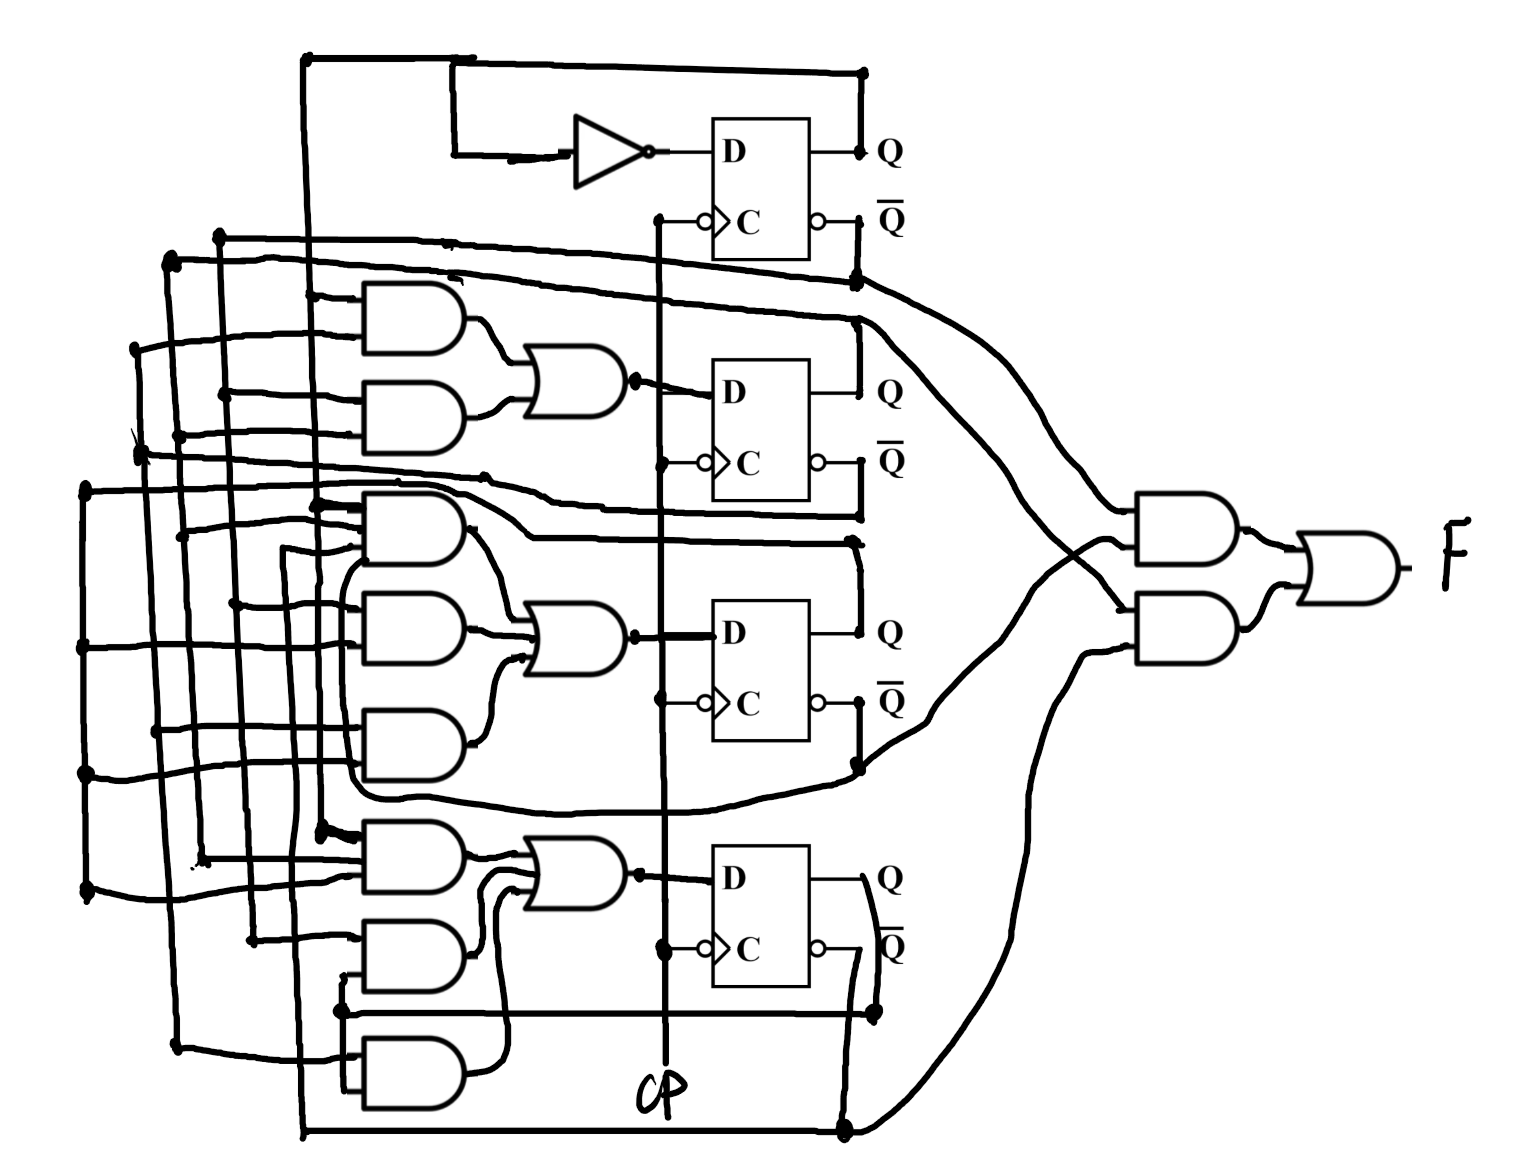
\includegraphics[width=0.4\textwidth]{image/electrical_18.png}\end{center}
\end{Answer}

\begin{question}{}{}
  6-21 Draw logic diagram, write the verilog code, and run the simulation.
\end{question}
\begin{Answer}
由题目易得，逻辑图如下：

\begin{center}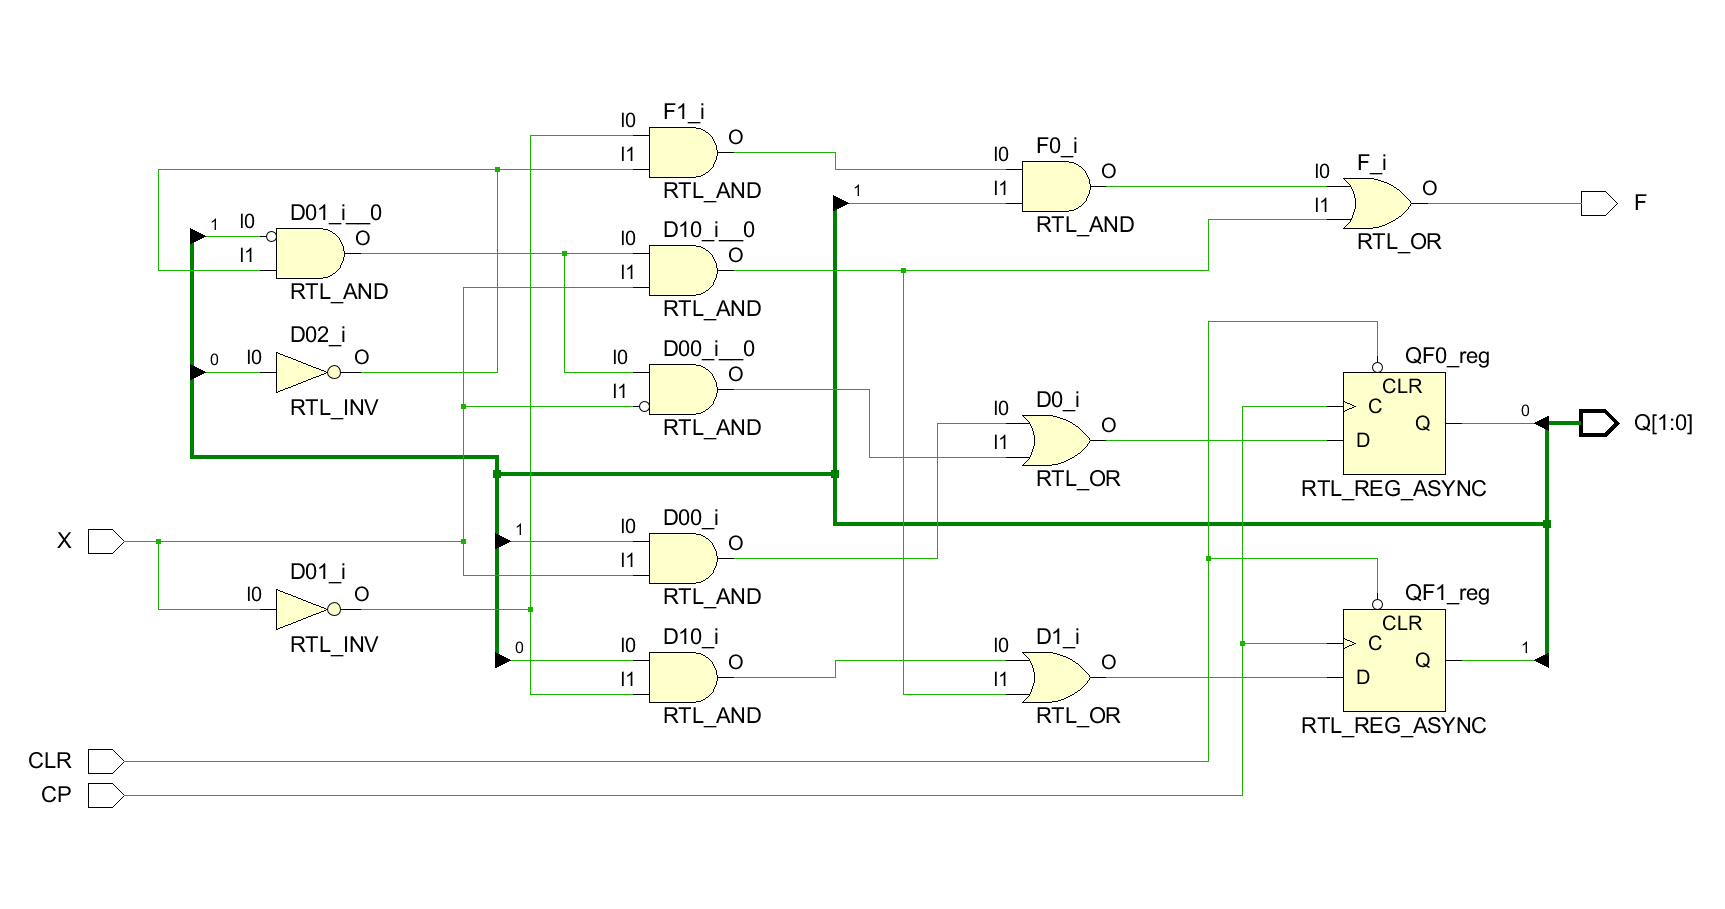
\includegraphics[width=0.6\textwidth]{image/electrical_19.png}\end{center}

下面是一个用于仿真Verilog模块的测试程序：

\begin{verilogcode}[caption={Verilog: 21}]
`timescale 1ns/1ps

module T6_21_tb;
    reg X;
    reg CP;
    reg CLR;
    wire F;
    wire [1:0] Q;
    T6_21 dut (
        .X(X),
        .CP(CP),
        .CLR(CLR),
        .F(F),
        .Q(Q)
    );
    initial begin
        CP = 0;
        forever #5 CP = ~CP;
    end
    initial begin
        $dumpfile("tb.vcd");
        $dumpvars(0, T6_21_tb);
        CLR = 0;
        X = 0;
        #10 CLR = 1;
        #10 X = 1;
        #10 X = 0;
        #10 X = 1;
        #10 X = 0;
        #20 X = 1;
        #20 X = 0;
        #100 $finish;
    end
endmodule
\end{verilogcode}

从代码中可以看出，这是一个由 QF0 和 QF1 组成的有限状态机（FSM）。
状态转移和输出 F 的生成都依赖于 X 的值和当前状态。

通过观察 D0 和 D1 的计算方式，以及 F 的生成逻辑，可以推测其行为类似于一种序列检测器或某种特定功能的状态机。
具体功能根据图片得到类似二进制和三进制转化计数器。

通过仿真可以验证该设计的行为并观察在不同输入序列下的状态变化和输出结果。
通过波形进行分析，进一步理解电路的具体功能和时序特性，如图所示：

\begin{center}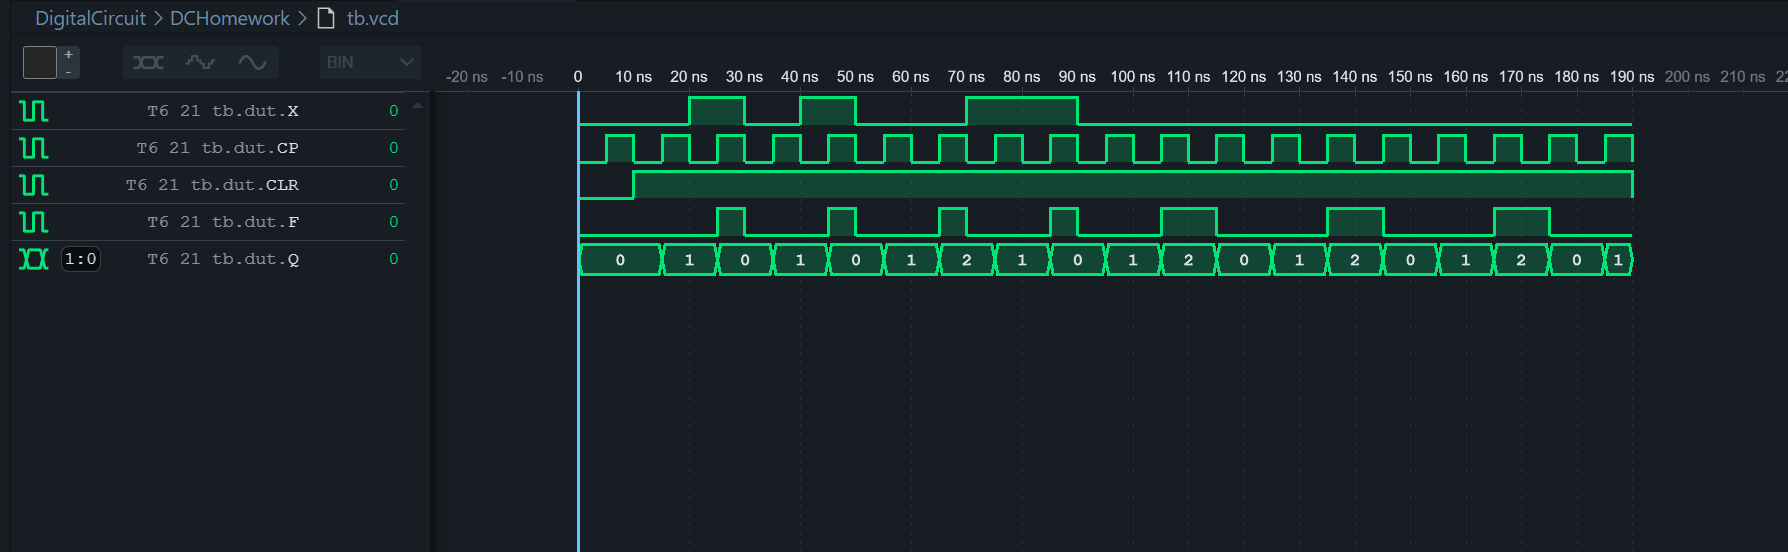
\includegraphics[width=0.8\textwidth]{image/wave_10.png}\end{center}
\end{Answer}

\begin{question}{}{}
  6-22 Draw logic diagram, write the verilog code, and run the simulation.
\end{question}
\begin{Answer}
由题目易得，逻辑图如下：

\begin{center}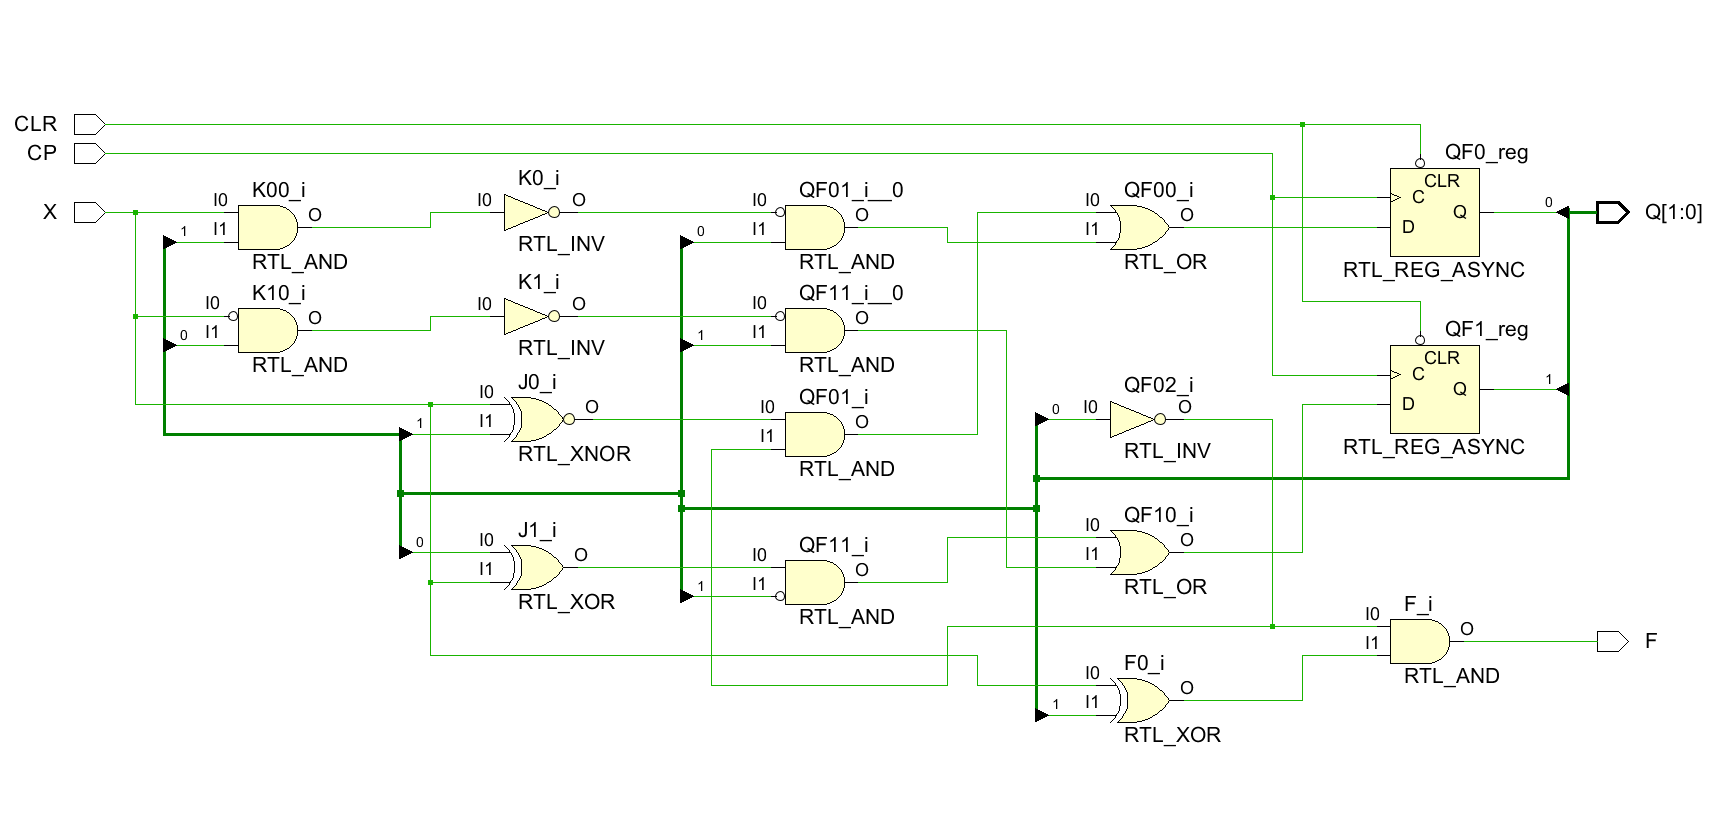
\includegraphics[width=0.6\textwidth]{image/electrical_20.png}\end{center}

下面是一个用于仿真Verilog模块的测试程序：

\begin{verilogcode}[caption={Verilog: 22}]
`timescale 1ns/1ps

module T6_22_tb;
    reg X;
    reg CP;
    reg CLR;
    wire F;
    wire [1:0] Q;
    T6_22 dut (
        .X(X),
        .CP(CP),
        .CLR(CLR),
        .F(F),
        .Q(Q)
    );
    initial begin
        CP = 0;
        forever #20 CP = ~CP;
    end
    initial begin
        X = 0;
        CLR = 0;
        $dumpfile("tb.vcd");
        $dumpvars(0, T6_22_tb);
        #10 CLR = 1;
        #230 X = 1;
        #200 X = 0;
        #60 $finish;
    end
endmodule
\end{verilogcode}

该电路实现了一个基于两个JK触发器的复杂状态机，
其状态和输出受输入X和时钟CP的控制，
并且可以通过CLR信号清零。

如图所示：
\begin{center}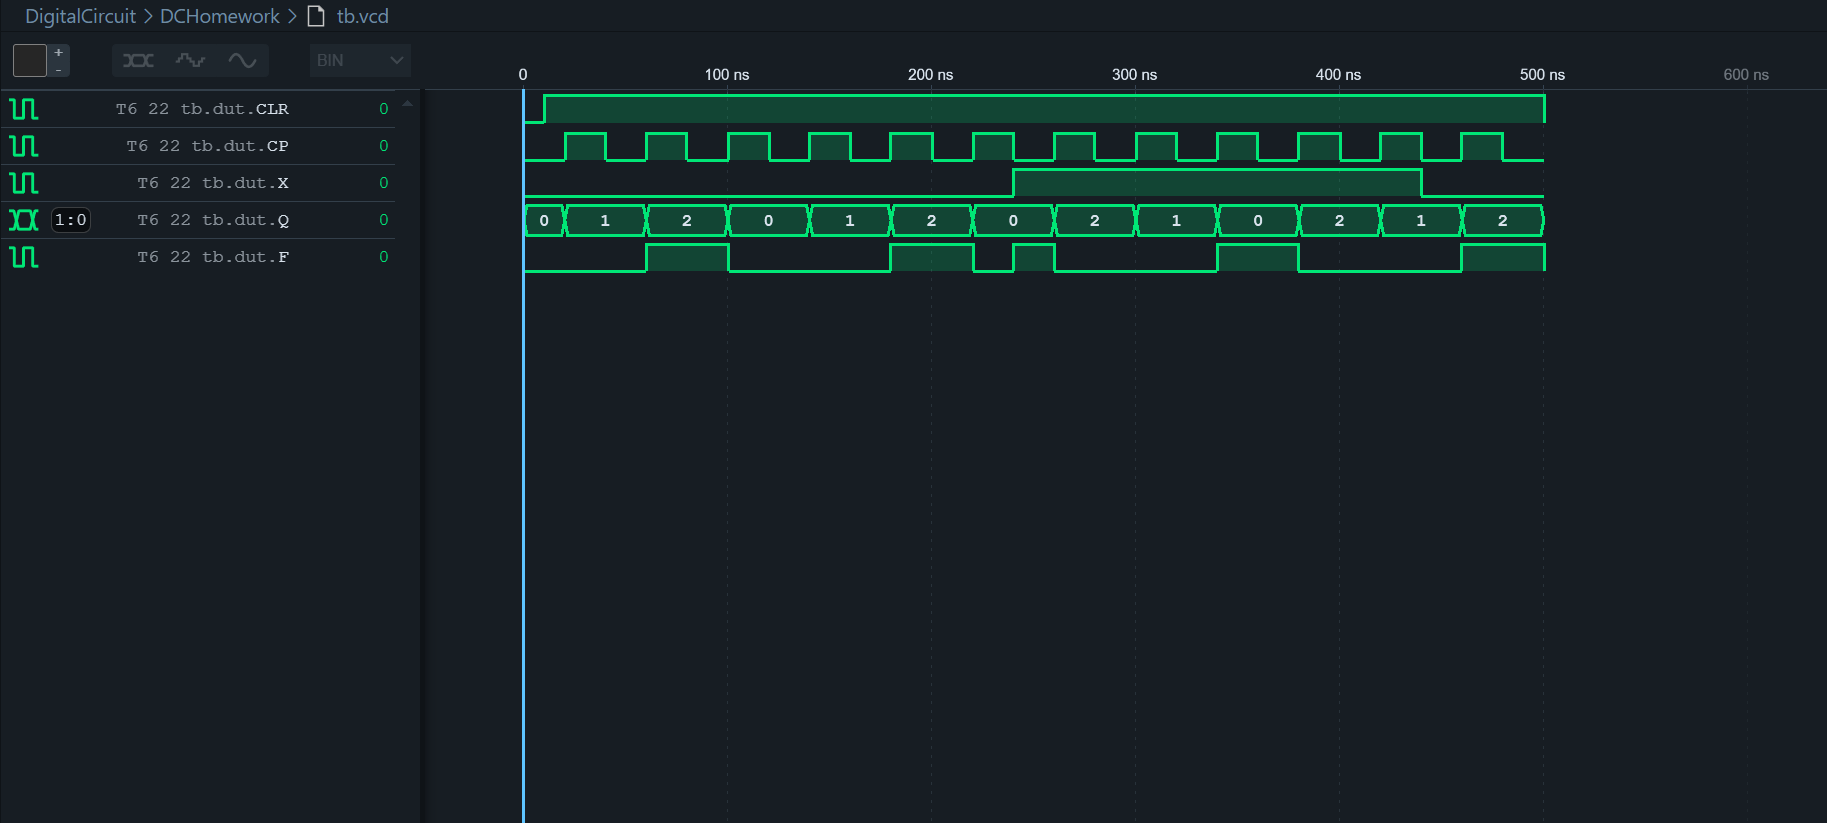
\includegraphics[width=0.8\textwidth]{image/wave_11.png}\end{center}

可知该器件实现了根据输入决定三进制的增加计数还是减少计数的功能。
\end{Answer}

\begin{question}{}{}
  6-23 Draw logic diagram and state transition diagram, write the verilog code, and run the simulation.
\end{question}
\begin{Answer}
由题目易得，逻辑图如下：

\begin{center}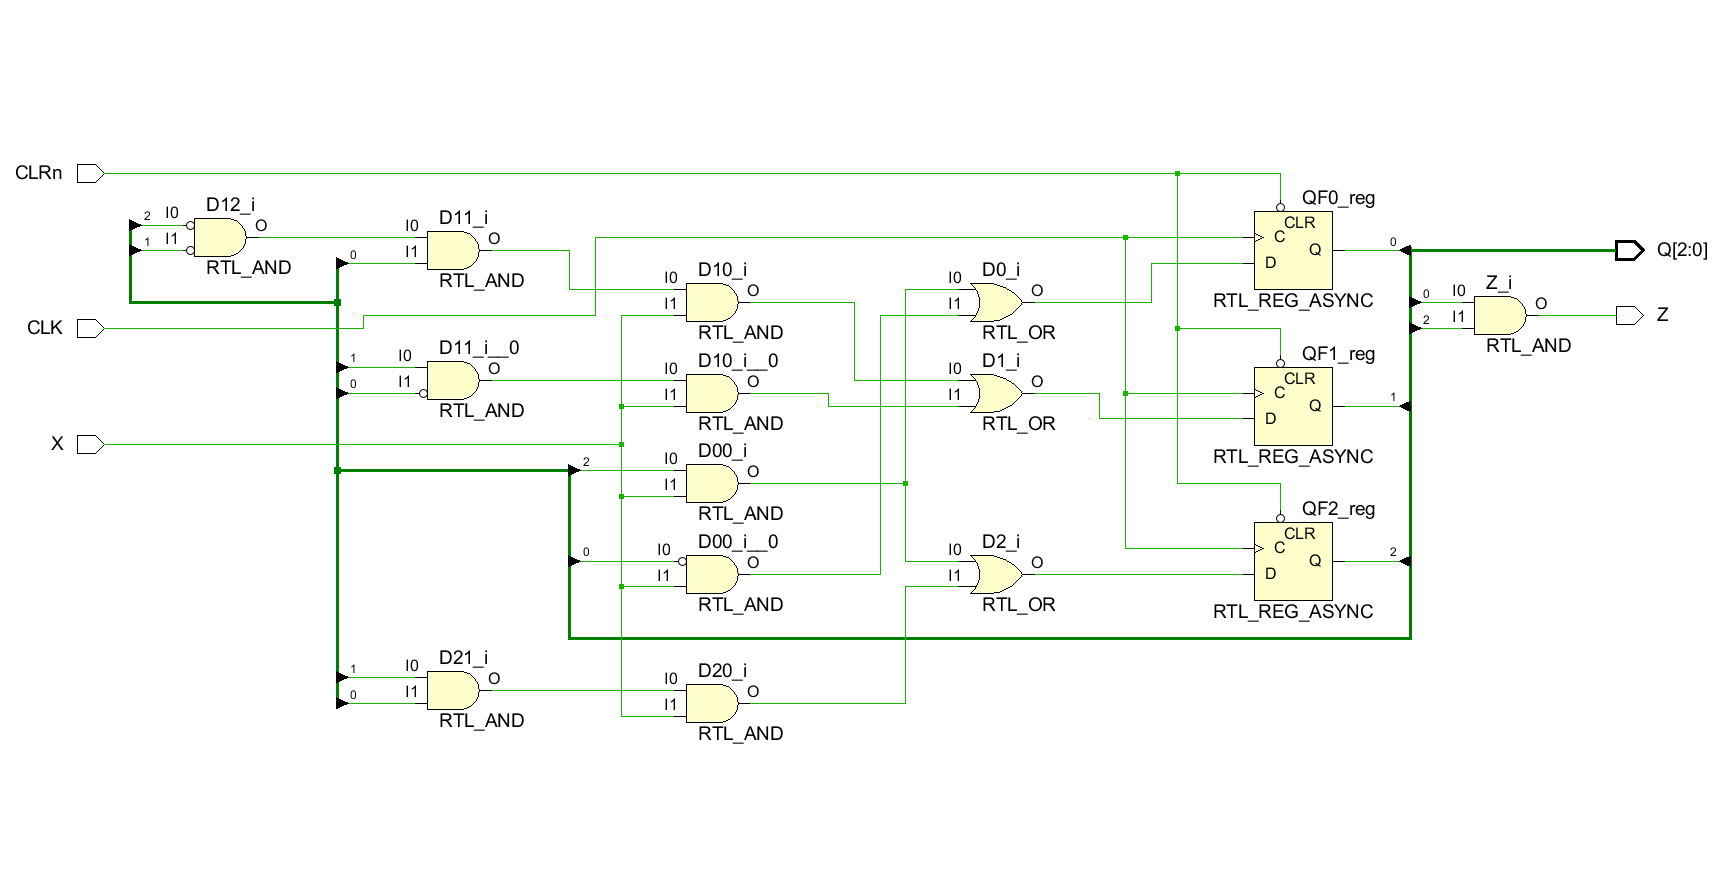
\includegraphics[width=0.6\textwidth]{image/electrical_21.png}\end{center}

状态转化图如下：

\begin{center}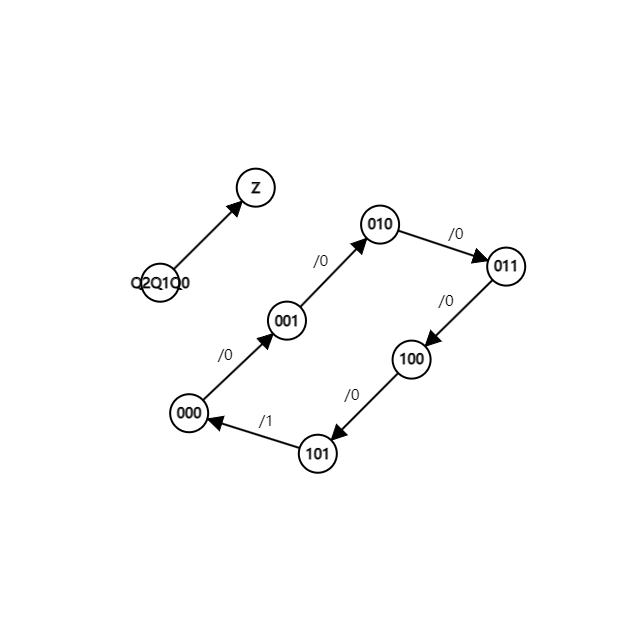
\includegraphics[width=0.4\textwidth]{image/graph_6.png}\end{center}

下面是一个用于仿真Verilog模块的测试程序：

\begin{verilogcode}[caption={Verilog: 23}]
`timescale 1ns/1ps

module T6_22_tb;
    reg X;
    reg CP;
    reg CLR;
    wire F;
    wire [1:0] Q;
    T6_22 dut (
        .X(X),
        .CP(CP),
        .CLR(CLR),
        .F(F),
        .Q(Q)
    );
    initial begin
        CP = 0;
        forever #5 CP = ~CP;
    end
    initial begin
        X = 0;
        CLR = 0;
        $dumpfile("tb.vcd");
        $dumpvars(0, T6_22_tb);
        #10 CLR = 1;
        #10 X = 1;
        #10 X = 0;
        #10 X = 1;
        #10 X = 0;
        #100 $finish;
    end
endmodule
\end{verilogcode}

该模块实现了一个三位状态机，其中状态的转移由输入X和当前状态（即寄存器QF0、QF1、QF2）决定。
输出Z表示当前状态中QF0和QF2均为1时的状态。

通过仿真，可以更好地观察该状态机的行为，并验证其正确性。
如图所示：

\begin{center}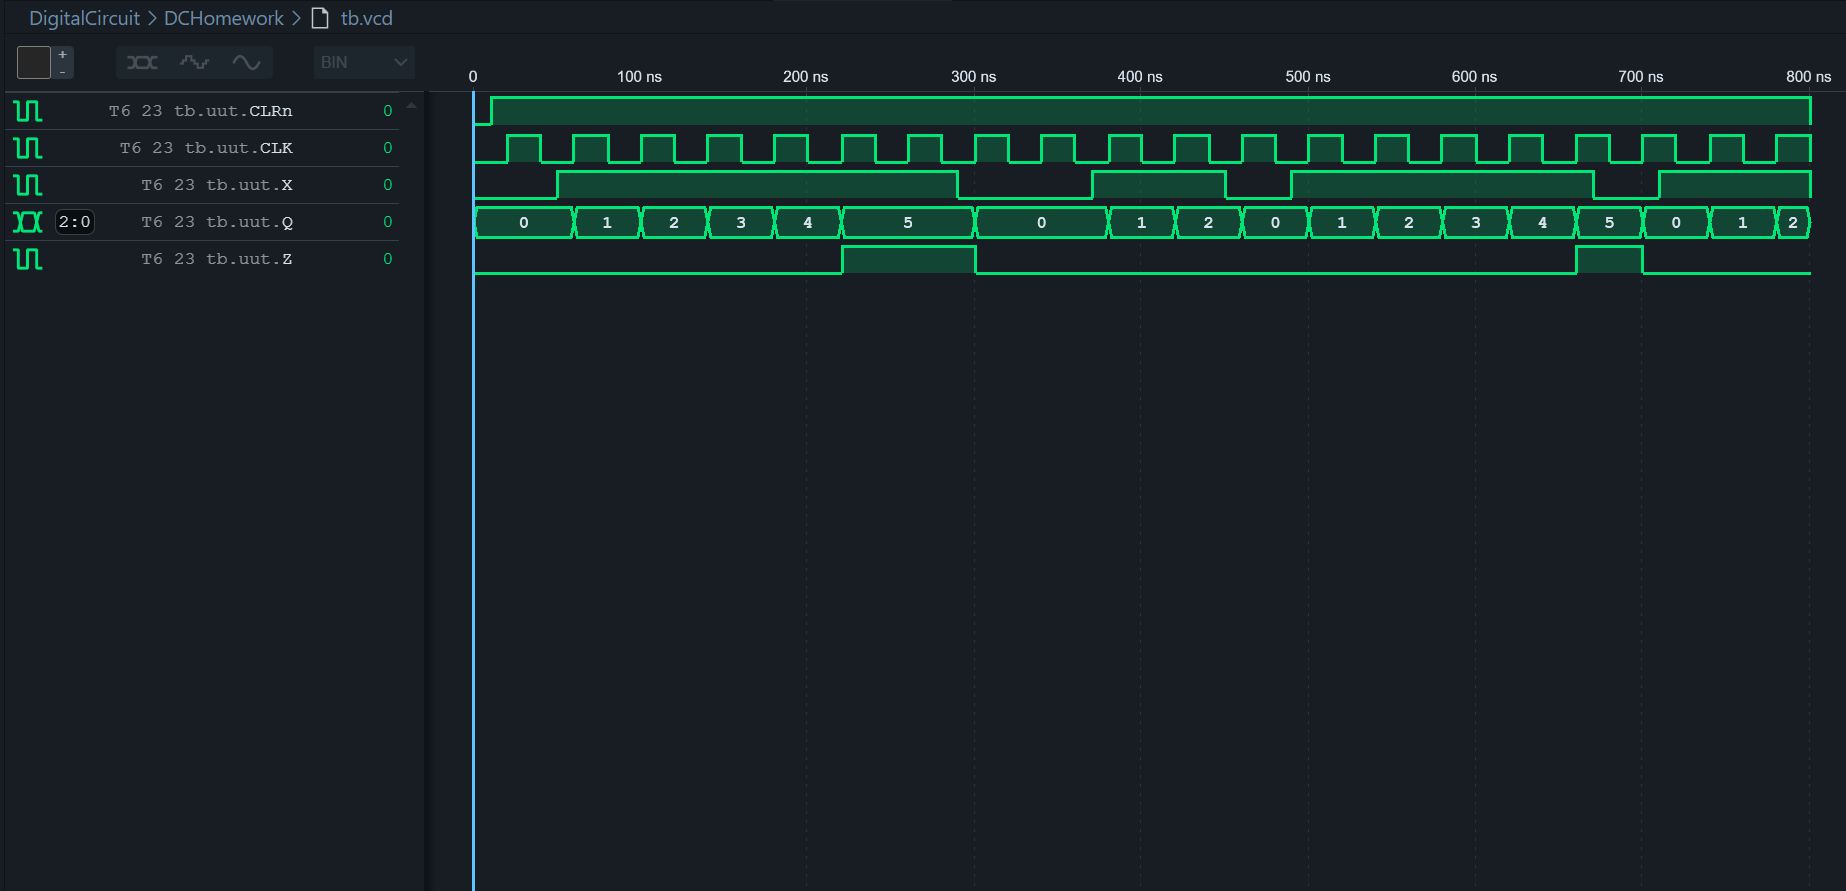
\includegraphics[width=0.8\textwidth]{image/wave_12.png}\end{center}

可知该器件实现了六进制计数功能。
\end{Answer}

\begin{question}{}{}
  6-24 Draw logic diagram and state transition diagram, write the verilog code, and run the simulation.
\end{question}
\begin{Answer}
由题目易得，逻辑图如下：

\begin{center}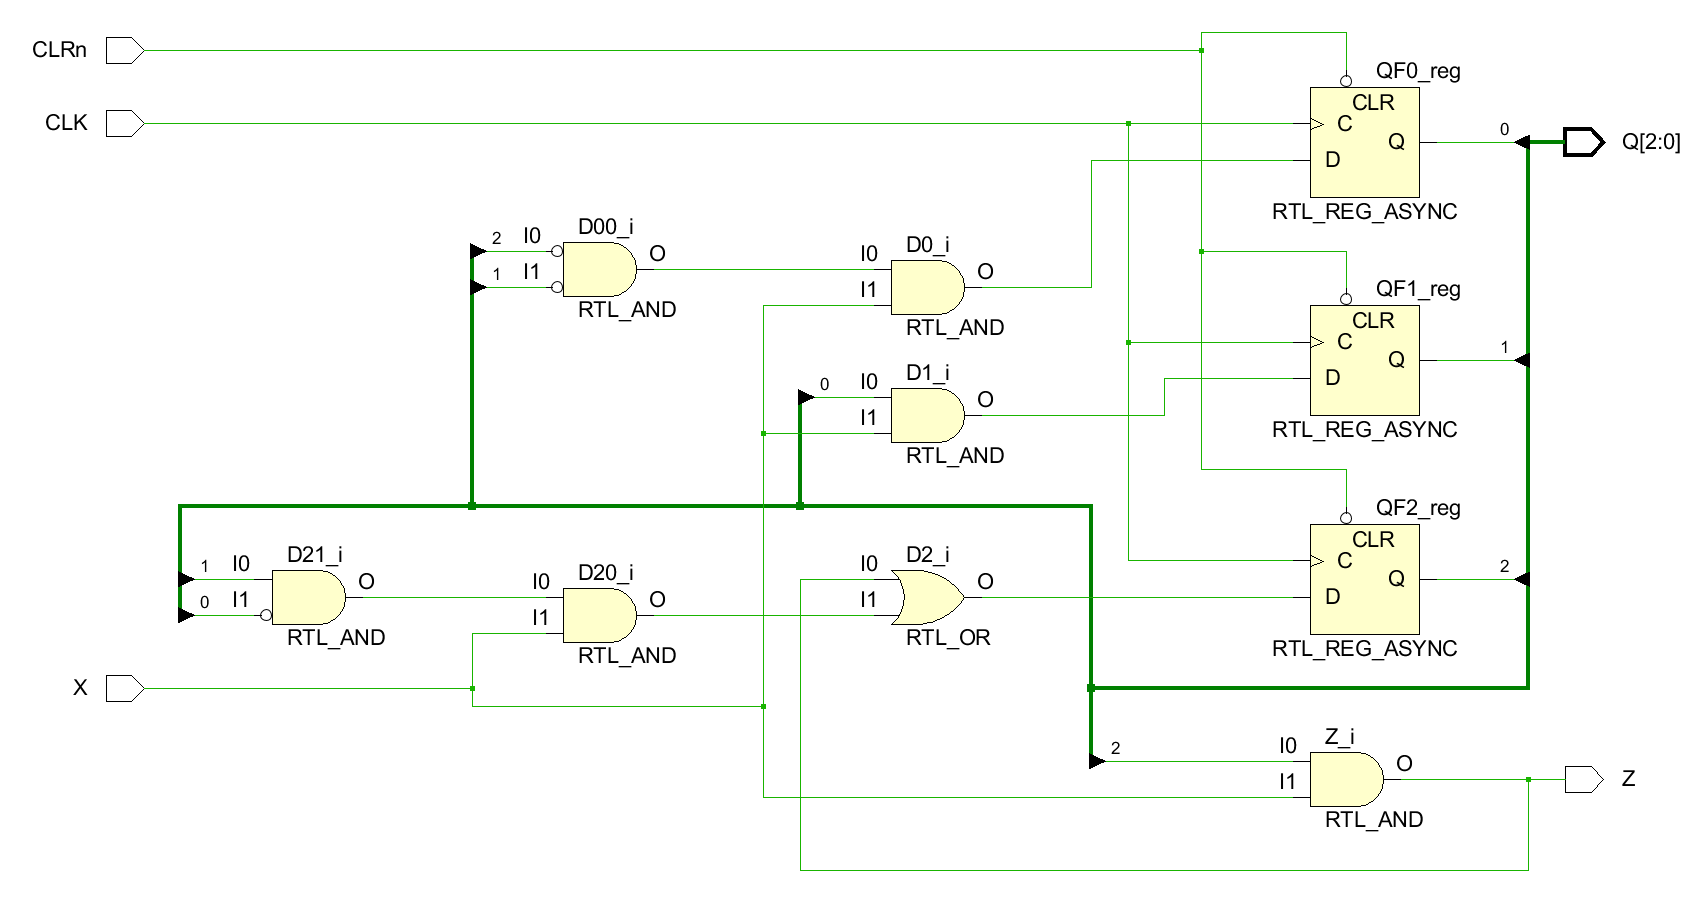
\includegraphics[width=0.6\textwidth]{image/electrical_22.png}\end{center}

状态转化图如下：

\begin{center}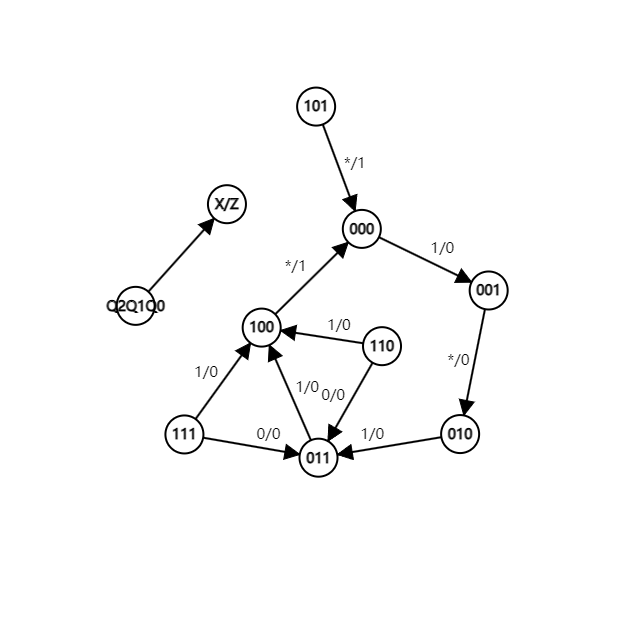
\includegraphics[width=0.4\textwidth]{image/graph_7.png}\end{center}

下面是一个用于仿真Verilog模块的测试程序：

\begin{verilogcode}[caption={Verilog: 24}]
`timescale 1ns/1ps

module T6_24_tb;
    reg X;
    reg CLK;
    reg CLRn;
    wire Z;
    wire [2:0] Q;
    T6_24 uut (
        .X(X),
        .CLK(CLK),
        .CLRn(CLRn),
        .Z(Z),
        .Q(Q)
    );
    initial begin
        CLK = 0;
        forever #20 CLK = ~CLK;
    end
    initial begin
        X = 0;
        CLRn = 0;
        $dumpfile("tb.vcd");
        $dumpvars(0, T6_24_tb);
        #10 CLRn = 1;
        #40 X = 1;
        #240 X = 0;
        #80 X = 1;
        #80 X = 0;
        #40 X = 1;
        #180 X = 0;
        #40 X = 1;
        #90 $finish;
    end
endmodule
\end{verilogcode}

该模块实现了一个三位状态机，其中状态的转移由输入X和当前状态（即寄存器QF0、QF1、QF2）决定。
输出Z表示当前状态中QF0和QF2均为1时的状态。

通过仿真，可以更好地观察该状态机的行为，并验证其正确性。
如图所示：

\begin{center}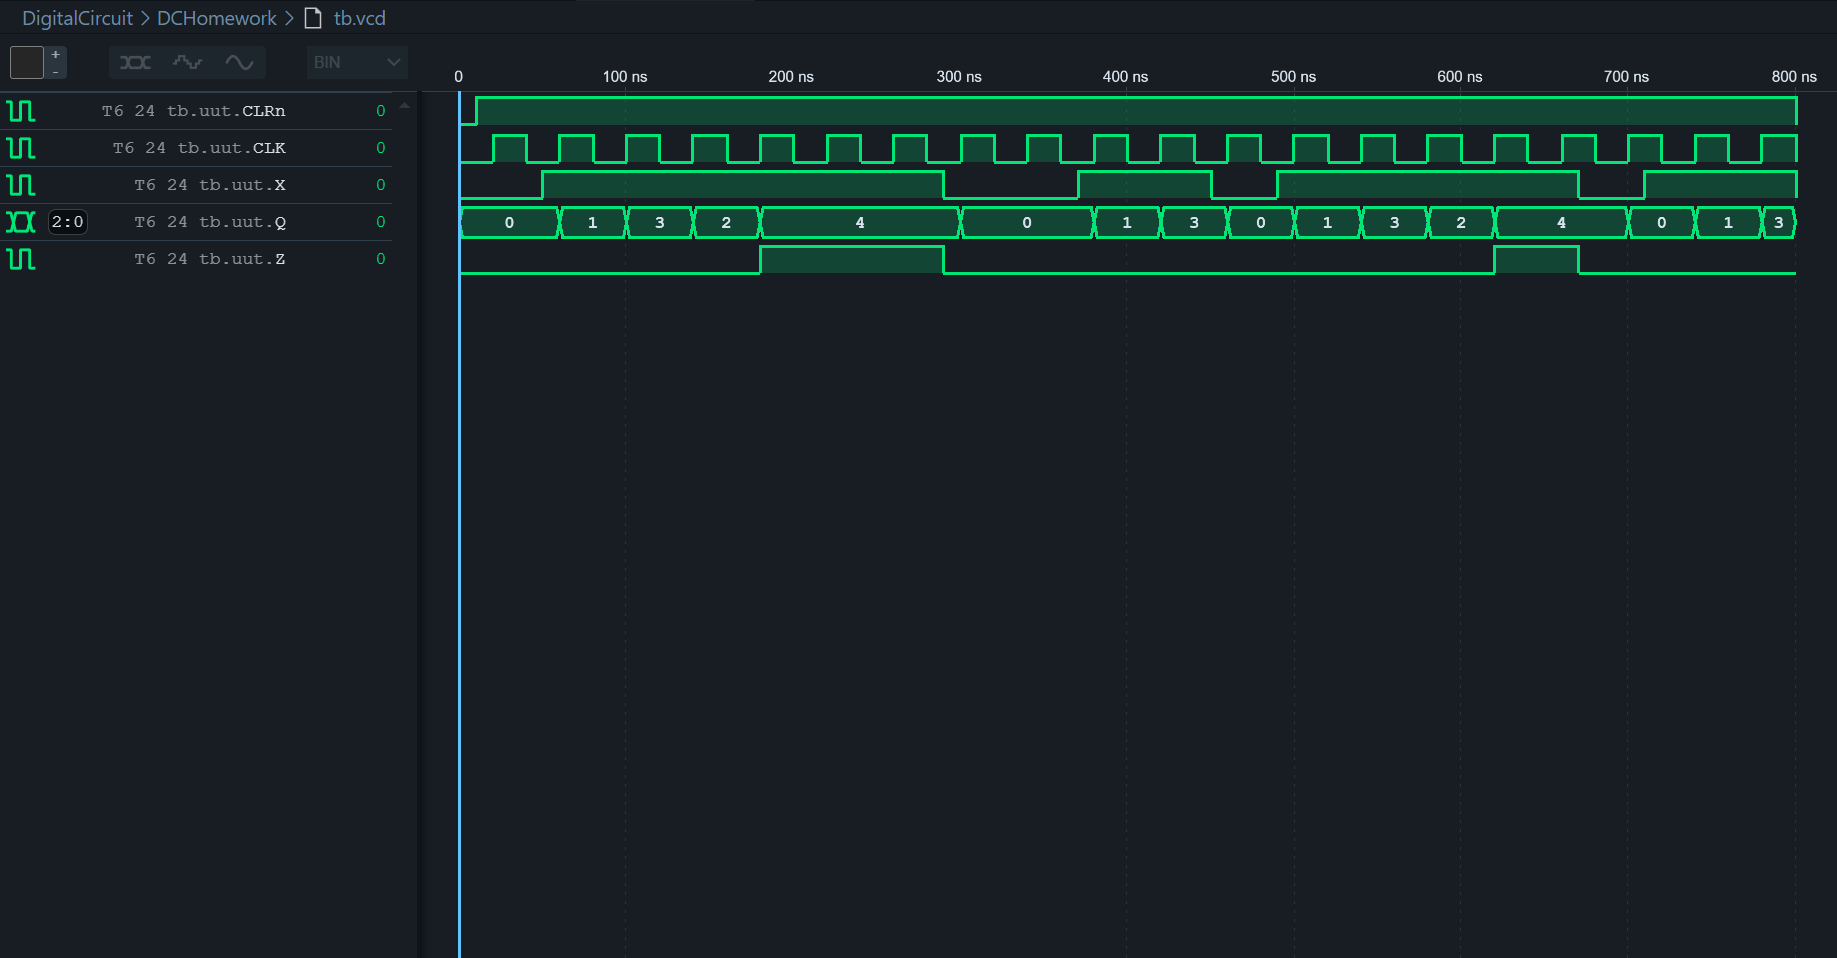
\includegraphics[width=0.8\textwidth]{image/wave_13.png}\end{center}

可知，该器件与上一题不同的是，该器件实现的是五进制计数功能。
\end{Answer}

\begin{question}{}{}
  6-25 Draw state transition diagram, and run the simulation.
\end{question}
\begin{Answer}
由题目易得，状态转化图如下：

\begin{center}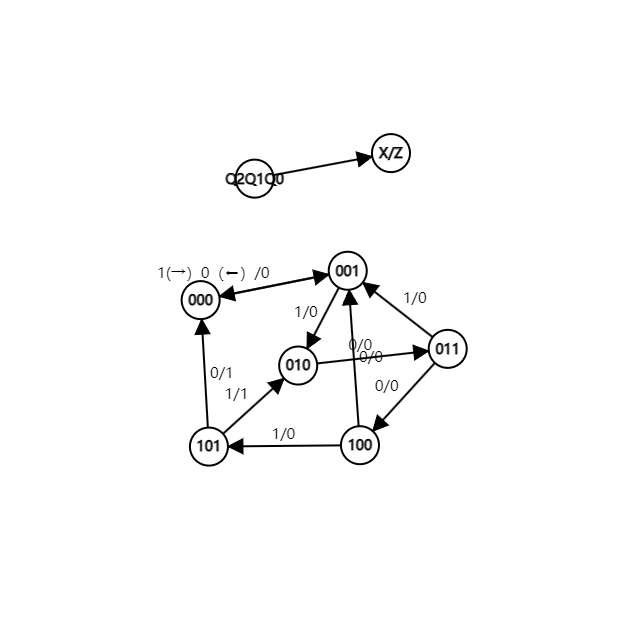
\includegraphics[width=0.4\textwidth]{image/graph_8.png}\end{center}

该Verilog模块实现了一个有限状态机（FSM），
通过仿真，我们能够观察状态机的状态转移和输出信号Z的变化。
输出波形如图所示：

\begin{center}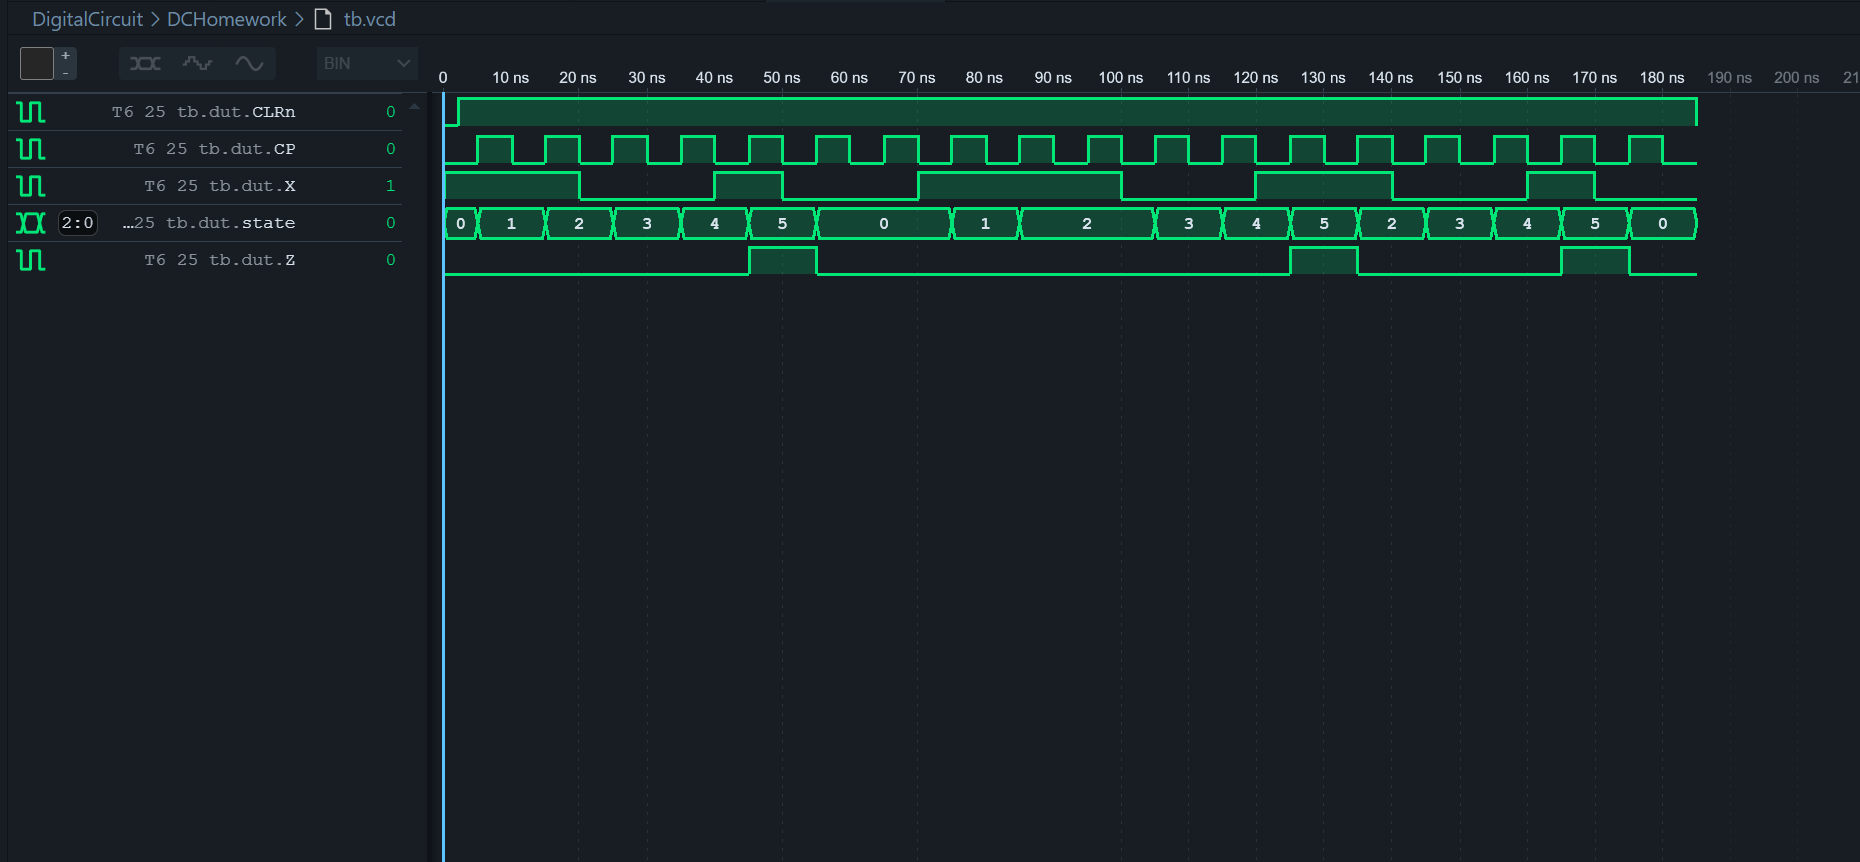
\includegraphics[width=0.8\textwidth]{image/wave_14.png}\end{center}

可知，该器件可以检测多种序列，
具体而言实现的是$((10)^*11001)$序列检测器。
\end{Answer}

\begin{question}{}{}
  6-26 Analyze the functions and run the simulation.
\end{question}
\begin{Answer}
该Verilog程序定义了一个名为T6\_26的模块，
该模块主要包含一个74LS194模块的实例。
74LS194是一个4位双向移位寄存器，
具有串行输入和并行输出。

该电路根据 S1 信号的状态控制移位寄存器的移位方向。
具体来说，当 S1 为0时，寄存器执行右移操作；
当 S1 为1时，寄存器执行左移操作。

输出波形如图所示：

\begin{center}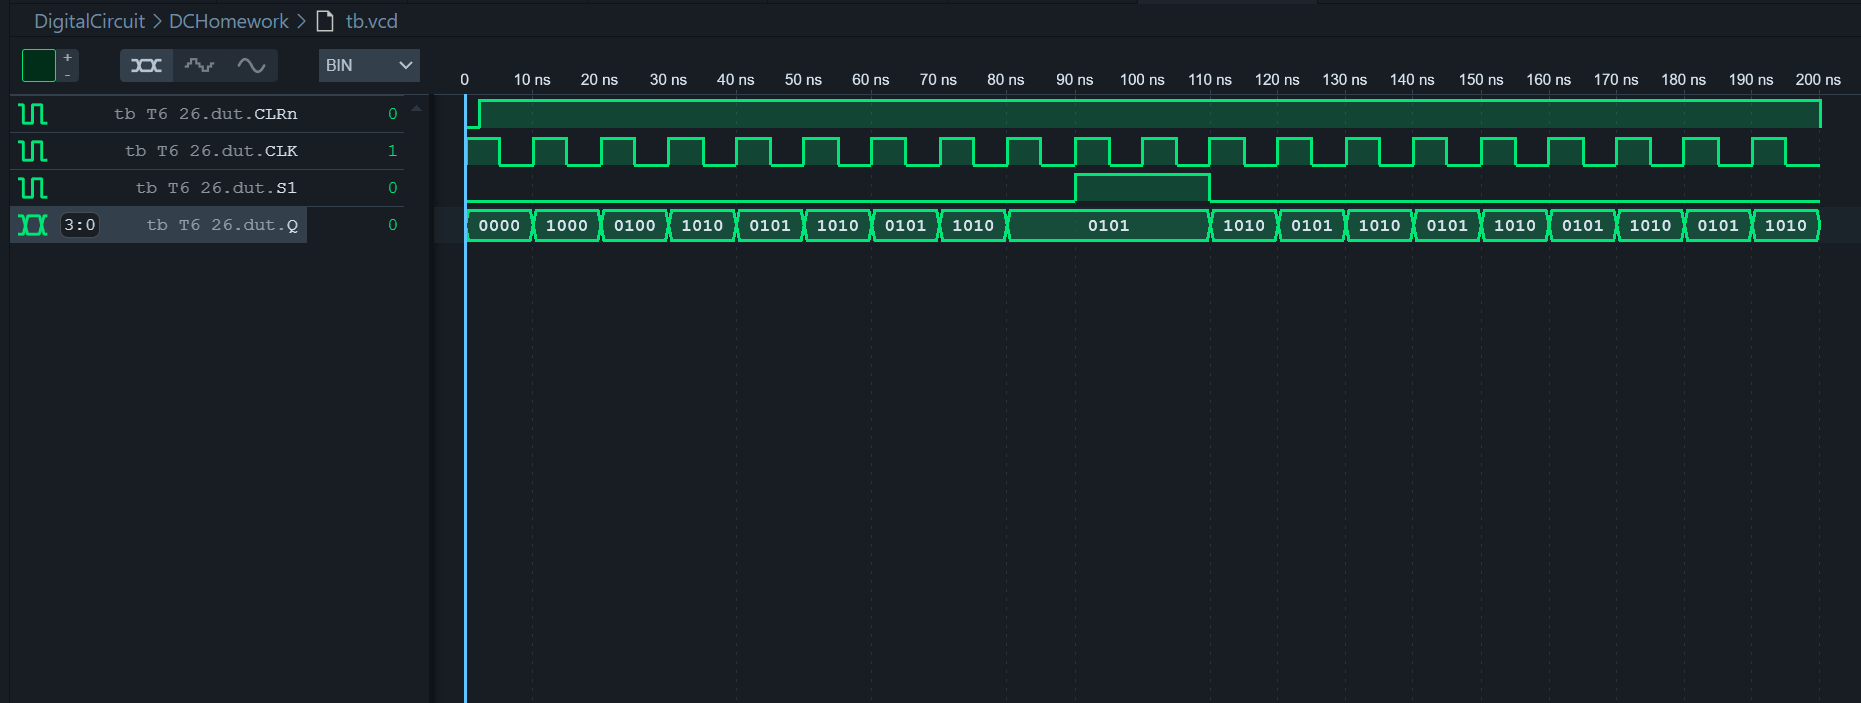
\includegraphics[width=0.8\textwidth]{image/wave_15.png}\end{center}

T6\_26模块通过S1控制移位寄存器的移位方向，
并且将右移输入连接为 ~Q[3]，
实现了一个有趣的逻辑功能。

具体而言，
该模块实现的是不断产生01序列并且右移。
\end{Answer}

\begin{question}{}{}
  6-27 Draw logic diagram and state transition diagram, and run the simulation.
\end{question}
\begin{Answer}
由题目易得，逻辑图如下：

\begin{center}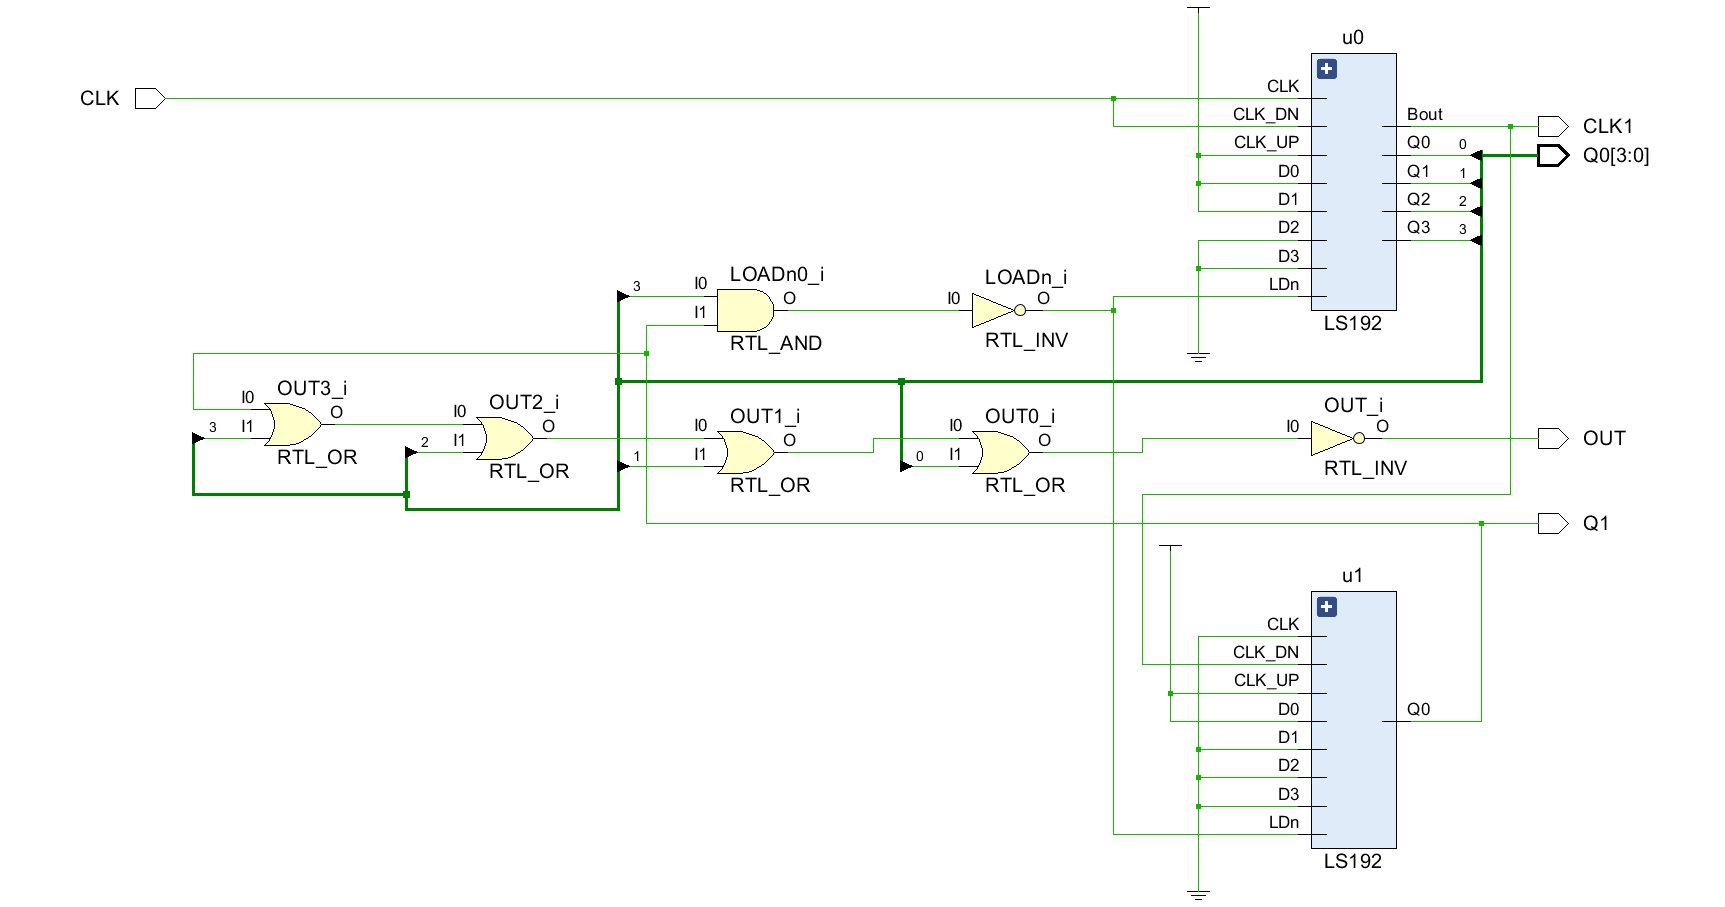
\includegraphics[width=0.6\textwidth]{image/electrical_23.png}\end{center}

状态转化图如下：

\begin{center}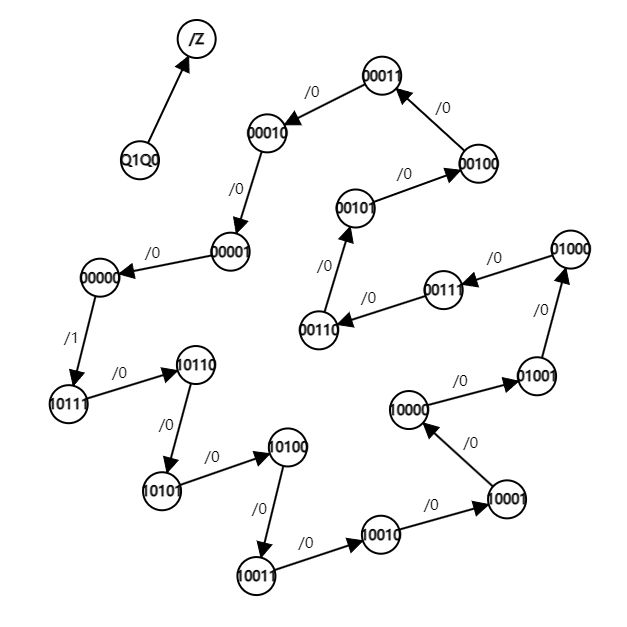
\includegraphics[width=0.4\textwidth]{image/graph_9.png}\end{center}

该模块通过实例化两个74LS192计数器实现了一个特定功能的逻辑电路。
74LS192是一个二进制计数器，具有同步加载和递增/递减功能。

如图所示：

\begin{center}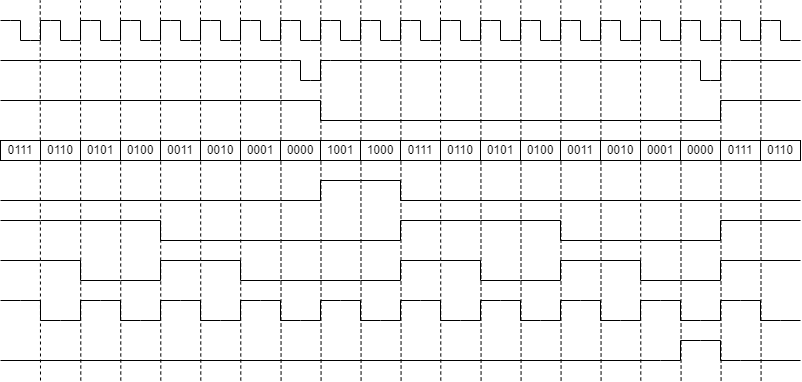
\includegraphics[width=0.8\textwidth]{image/wave_16.png}\end{center}

T6\_27模块通过两个74LS192计数器实现了分频计数和特定状态输出。
该器件是一个十八位进制减法计数器。
\end{Answer}

\begin{question}{}{}
  6-28 Draw logic diagram and state transition diagram, and run the simulation.
\end{question}
\begin{Answer}
由题目易得，逻辑图如下：

\begin{center}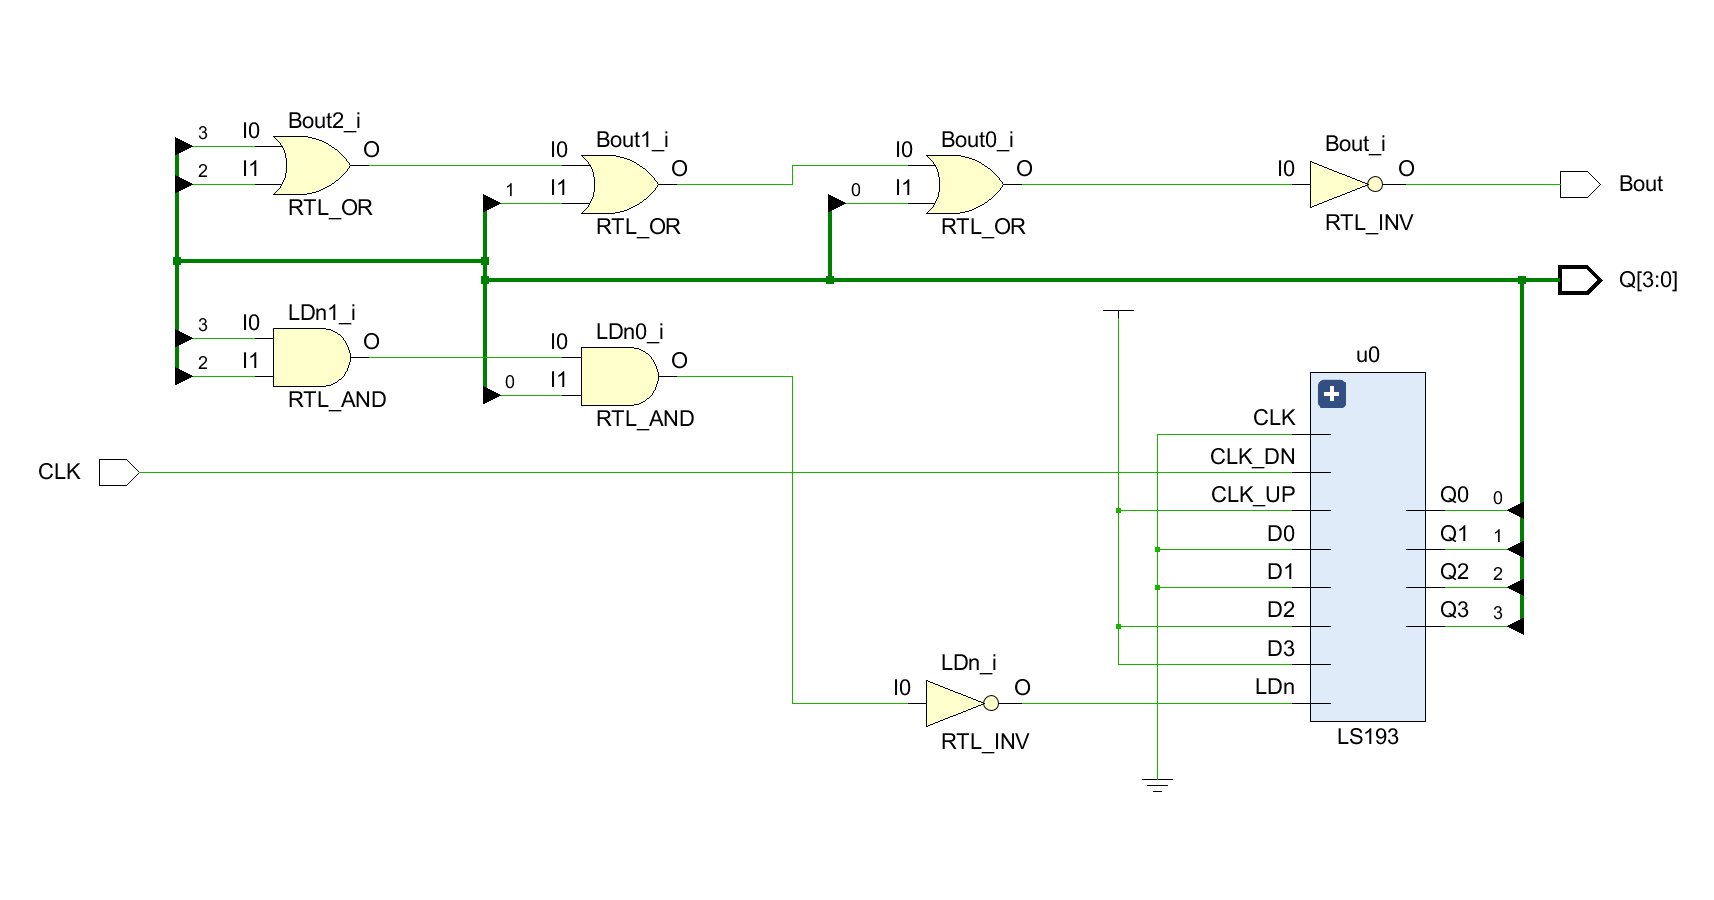
\includegraphics[width=0.6\textwidth]{image/electrical_24.png}\end{center}

状态转化图如下：

\begin{center}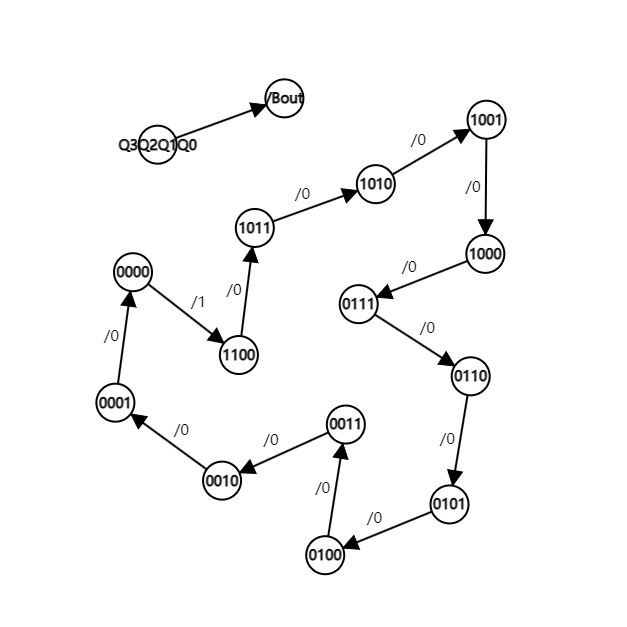
\includegraphics[width=0.4\textwidth]{image/graph_10.png}\end{center}

该Verilog模块 T6\_28 实现了一个计数器功能，
具体来说是使用 74LS193 作为计数器核。

如图所示：

\begin{center}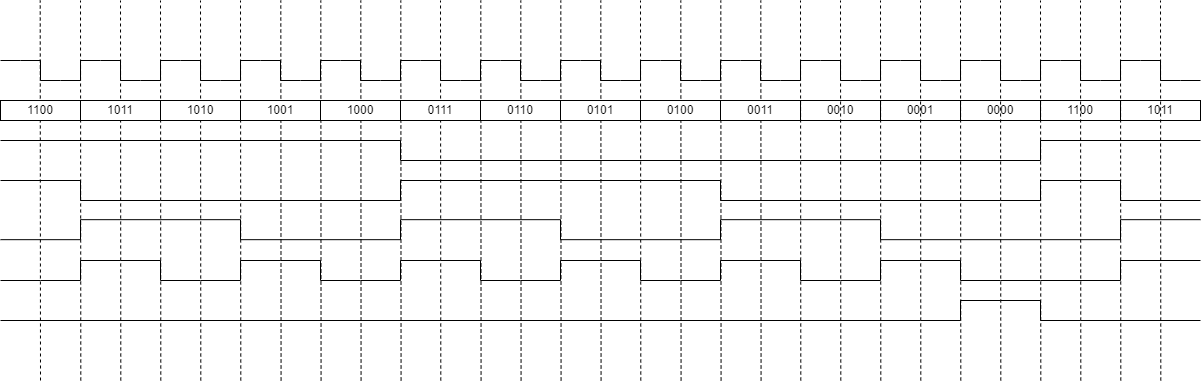
\includegraphics[width=0.8\textwidth]{image/wave_17.png}\end{center}

该逻辑电路的功能是使用74LS193作为计数器，
当计数值到达特定值（如全1或全0）时，
输出对应的标志位，
并根据时钟信号进行加计数或减计数。
可知该器件是一个十三位进制减法计数器。
\end{Answer}

\begin{question}{}{}
  6-29 Analyze the functions.
\end{question}
\begin{Answer}
由题目易得，该模块实现了循环六位左移计数寄存器，
最高位为1时输出F。
\end{Answer}

\begin{flushright}\begin{tabular}{rl}
  姓名: & 李俊洁\\
  班级: & 计算机2204 \\
  学号: & 20225443 \\
  课程: & 数字逻辑与数字系统 \\
  日期: & June 15, 2024 \\
  制作: & \LaTeX \\
  & 感谢您的批阅！
\end{tabular}\end{flushright}
\end{document}
